\documentclass[../DoAn.tex]{subfiles}

\begin{document}

\section{Thiết kế kiến trúc}
\label{section:systemdesign}

\subsection{Lựa chọn kiến trúc phần mềm}
\label{subsection:systemdesign-architecture}
% Mục này có độ dài từ một đến ba trang. Sinh viên cần lựa chọn kiến trúc phần mềm cho ứng dụng của mình như: kiến trúc ba lớp MVC, MVP, SOA, Microservice, v.v. rồi giải thích sơ bộ về kiến trúc đó (không giải thích chi tiết/dài dòng).
% Sử dụng kiến trúc phần mềm đã chọn ở trên, sinh viên mô tả kiến trúc cụ thể cho ứng dụng của mình. Gợi ý: sinh viên áp dụng lý thuyết chung vào hệ thống/sản phẩm của mình như thế nào, có thay đổi, bổ sung hoặc cải tiến gì không. Ví dụ, thành phần M trong kiến trúc lý thuyết MVC sẽ là những thành phần cụ thể nào (ví dụ: là interface I + class C1 + class C2, v.v.) trong kiến trúc phần mềm của sinh viên.
Trong thiết kế hệ thống thông tin, ta thường biết đến rất nhiều cách tiếp cận, thiết kế và cấu trúc dự án khác nhau. Sau khi xem xét kĩ lưỡng, mô hình Client-Server sẽ làm hệ thống có tính mở rộng cao và dễ dàng truy cập. Khi đó dữ liệu của hệ thống sẽ là một server riêng biệt, còn phần giao diện và thao tác dữ liệu sẽ là một hoặc nhiều kiểu client riêng biệt. Với mục tiêu đó, một bộ API sẽ được xây dựng cùng với cơ sở dữ liệu được đóng gói trong một server có thể được host trên các dịch vụ cloud hoặc thậm chí home server. Về phía Client hiện giờ sẽ được phát triển là một ứng dụng di động để người dùng dễ dàng thao tác nhất.

Khi thiết kế \textbf{Server}, kiểu hệ thống Monolithic và Microservice là hai cách tiếp cận phổ biến nhất. Tuy nhiên, với đối tượng người dùng là các hộ kinh doanh vừa và nhỏ, việc sử dụng Microservice sẽ quá phức tạp và thêm nhiều phần xử lí thừa. Do đó, kiểu Monolithic sẽ tối giản quá trình phát triển và đẩy nhanh tiến độ rất nhiều. Thiết kế sẽ bao gồm các đầu API cùng với logic xử lí và truy cập lưu trữ cơ sở dữ liệu vào trong một process. Hình \ref{fig:MonolithVsMicroservices}  mô tả sự khác biệt giữa hai kiểu kiến trúc này.
\begin{figure}[H]
    \centering
    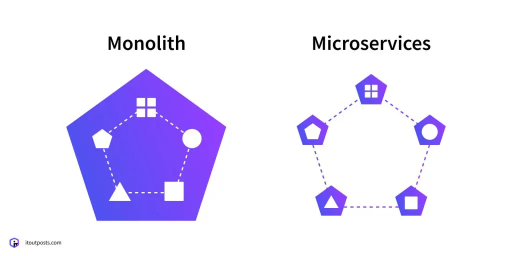
\includegraphics[width=0.8\textwidth]{Hinhve/design/architecture/MonolithVsMicroservices}
    \caption{Kiến trúc Monolithic và Microservice \cite{monovsmicroitoutposts}}
    % https://itoutposts.com/blog/monolith-vs-microservices-which-is-better-to-choose/
    \label{fig:MonolithVsMicroservices}
\end{figure}
\vfill
\break

Đi sâu hơn, khi tiếp cận việc thiết kế một bộ mã nguồn tường minh và dễ phát triển, kiến trúc N-tier (hình \ref{fig:NtierArchitecture}), Clean Architecture (hình \ref{fig:CleanArchitecture}) được đề xuất rất nhiều. Nhưng trong trường hợp thay đổi hệ cơ sở dữ liệu thì kiến trúc N-tier sẽ khiến ta phải cấu trúc lại rất nhiều vì tầng truy cập dữ liệu (Data Access Layer) nằm rất sâu trong hệ thống. Vì vậy, kiến trúc Clean Architecture sẽ được sử dụng trong hệ thống này vì nó trừu tượng hóa việc truy cập dữ liệu (Application Layer). Bất kể kiểu cơ sở dữ liệu nào, chúng sẽ đều phải kế thừa lớp trừu tượng đó, do đó giải quyết được vấn đề thay đổi công nghệ trong tương lai. Lựa chọn vì sao và thiết kế kiến trúc Clean Architecture sẽ được trình bày chi tiết ở phần \ref{section:clean_architecture}.
\begin{figure}[H]
    \begin{subfigure}{0.49\textwidth}
        \centering
        \includegraphics[width=0.8\linewidth]{Hinhve/design/architecture/NtierArchitecture}
        \caption{Kiến trúc N-tier \cite{aspnetntiercodeproject}}
        % https://www.codeproject.com/Articles/439688/Creating-ASP-NET-application-with-n-tier-architect
        \label{fig:NtierArchitecture}
    \end{subfigure}
    \begin{subfigure}{0.49\textwidth}
        \centering
        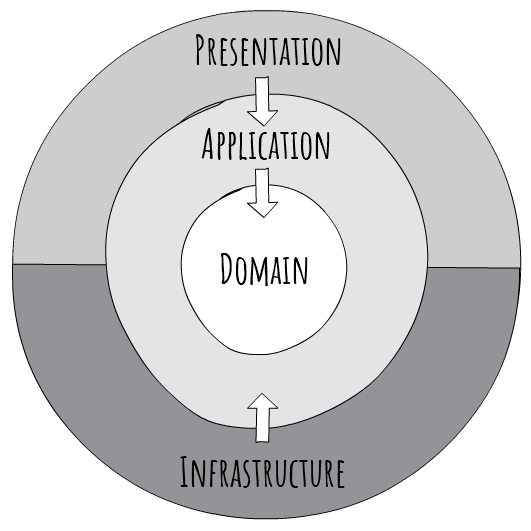
\includegraphics[width=0.6\linewidth]{Hinhve/design/architecture/CleanArchitecture}
        \caption{Kiến trúc Clean Architecture \cite{cleanarchitecturejasontaylor}}
        % https://jasontaylor.dev/clean-architecture-getting-started/
        \label{fig:CleanArchitecture}
    \end{subfigure}
    \caption{N-tier và Clean Architecture}
    \label{fig:NtiervsCleanArchitecture}
\end{figure}

Khi thiết kế \textbf{Client}, phổ biến nhất là các kiến trúc MVC, MVP... Nhưng kiến trúc MVVM (Model-View-ViewModel) (\ref{fig:MVVMArchitecture}) chứng minh được quy trình truyền tải dữ liệu giữa Model và View hiệu quả hơn nhiều. Kiến trúc này giúp phân tách rõ ràng giữa giao diện (View) và dữ liệu (Model) với một lớp trung gian (ViewModel) để xử lí logic và lan truyền hai chiều sự thay đổi trong dữ liệu. Điều này giúp cho việc phát triển ứng dụng di động trở nên dễ dàng hơn để kiểm thử, duy trì và mở rộng. Nó cũng giúp cải thiện việc sử dụng lại code và người thiết kế giao diện có thể làm việc độc lập với nhà phát triển logic. Chi tiết về lựa chọn và thiết kế kiến trúc MVVM sẽ được trình bày ở phần \ref{section:mvvm}.
\begin{figure}[H]
    \centering
    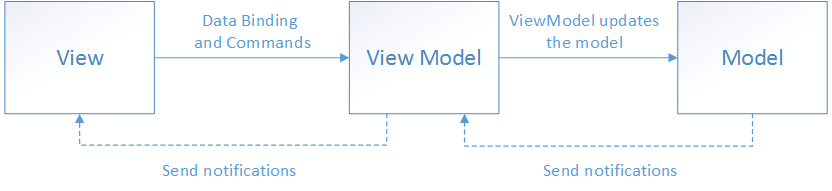
\includegraphics[width=0.8\textwidth]{Hinhve/design/architecture/MVVM}
    \caption{Kiến trúc MVVM \cite{mvvmmicrosoft}}
    % https://learn.microsoft.com/en-us/dotnet/architecture/maui/mvvm
    \label{fig:MVVMArchitecture}
\end{figure}
\break


\subsection{Thiết kế tổng quan}
\label{subsection:systemdesign-general}
% Sinh viên vẽ biểu đồ gói UML (UML package diagram), nêu rõ sự phụ thuộc giữa các gói (package). SV cần vẽ các gói sao cho chúng được phân theo các tầng rõ ràng, không được sắp đặt package lộn xộn trong hình vẽ. Sinh viên chú ý các quy tắc thiết kế (Các gói không phụ thuộc lẫn nhau, gói tầng dưới không phụ thuộc gói tầng trên, không phụ thuộc bỏ qua tầng, v.v.) và cần giải thích sơ lược về mục đích/nhiệm vụ của từng package. SV tham khảo ví dụ minh họa trong Hình \ref{fig:Fig1}
Hình \ref{fig:package} là biểu đồ gói tổng quan của hệ thống. Hệ thống được chia thành hai phần chính là \textbf{Server} và \textbf{Client}. Trong đó, \textbf{Server} sẽ chứa các thành phần liên quan đến logic xử lí và truy cập lưu trữ cơ sở dữ liệu. \textbf{Client} sẽ chứa các thành phần liên quan đến giao diện người dùng để giao tiếp với hệ thống.
\begin{figure}[H]
    \centering
    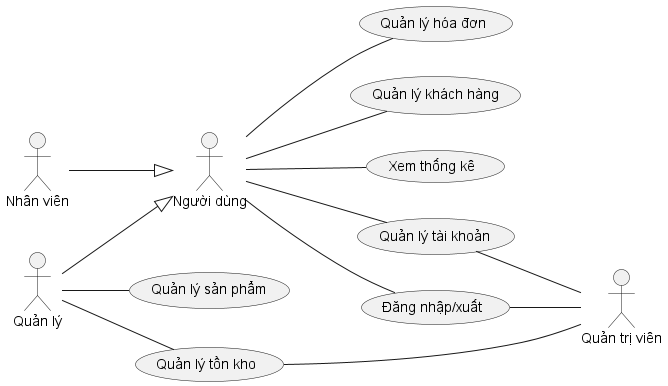
\includegraphics[width=0.8\textwidth]{Hinhve/design/package/General}
    \caption{Biểu đồ gói}
    \label{fig:package}
\end{figure}
\vfill
\break

Trong phần \textbf{Client}, hệ thống áp dụng mô hình MVVM và được chia thành các gói như sau:
\begin{itemize}
    \item \textbf{Views}: Gói này sẽ chứa các giao diện người dùng. Trong hệ thống này, nó sẽ chứa các màn hình như danh sách sản phẩm (ProductListPage), chi tiết sản phẩm (ProductDetailsPage), danh sách hóa đơn (InvoiceListPage),...
    \item \textbf{ViewModels}: Gói này sẽ chứa các thành phần liên quan đến logic xử lí và truyền tải dữ liệu giữa View và Model. Trong hệ thống này, ứng với mỗi trang sẽ có một ViewModel tương ứng. Ví dụ, trang danh sách sản phẩm sẽ có ProductListViewModel, trang chi tiết sản phẩm sẽ có ProductDetailsViewModel,...
    \item \textbf{HttpServices}: Gói này là tượng trưng cho lớp Model của mô hình MVVM. Chúng chứa các đối tượng gọi API để giao tiếp với hệ thống qua môi trường mạng. Trong hệ thống này, nó sẽ chứa các đối tượng hỗ trợ đăng nhập (IdentityService), quản lý sản phẩm (ProductService), quản lý hóa đơn (InvoiceService)...
\end{itemize}

Áp dụng kiến trúc \textbf{Clean Architecture} vào hệ thống, \textbf{Server} sẽ được chia thành các gói như sau:
\begin{itemize}
    \item \textbf{Presentation}: Gói này gồm các thành phần giao tiếp với hệ thống. Cụ thể, các gói \textbf{Controller} trong hệ thống này là các đầu API như đăng nhập (IdentityController), quản lý sản phẩm (ProductController), quản lý hóa đơn (InvoiceController)...
    \item \textbf{Application}: Gói này gồm các gói con như \textbf{Services, IRepositories}. Các gói \textbf{Services} mang nhiệm vụ lấy và lưu trữ dữ liệu từ gói \textbf{IRepositories} rồi xử lí các logic nghiệp vụ. Còn các gói \textbf{IRepositories} trừu tượng hóa các câu truy vấn cơ sở dữ liệu thành các hàm riêng. Mục đích này để cho dù dùng bất kì kiểu cơ sở dữ liệu nào (SQL Server, MongoDB) thì quy trình xử lí logic của hệ thống không bị ảnh hưởng.
    \item \textbf{Infrastructure}: Gói \textbf{Repositories} này sẽ kế thừa các gói \textbf{IRepositories} của gói \textbf{Application} và cài đặt các câu truy vấn với một hệ cơ sở dữ liệu nhất định. Trong hệ thống này sẽ dùng MongoDB nên gói này sẽ chứa các đối tượng kết nối và truy vấn cơ sở dữ liệu (MongoDatabase, ProductRepository, InvoiceRepository...).
    \item \textbf{Domain}: Gói \textbf{Entities} sẽ chứa các kiểu dữ liệu ứng với các bảng, các tài liệu được lưu trữ trong cơ sở dữ liệu. Chúng được định nghĩa bằng các lớp (User, Product, Invoice,...) và được sử dụng trong các gói \textbf{Repositories} và \textbf{Services}.
\end{itemize}
\break


\subsection{Thiết kế chi tiết gói}
\label{subsection:systemdesign-package}
% Sinh viên thiết kế và lần lượt vẽ biểu đồ thiết kế cho từng package, hoặc một nhóm các package liên quan để giải quyết một vấn đề gì đó. Khi vẽ thiết kế gói, sinh viên chỉ cần đưa tên lớp, không cần chỉ ra các thành viên phương thức và thuộc tính. SV tham khảo ví dụ minh họa trong Hình \ref{fig:Fig2}.

% Sinh viên cần vẽ rõ ràng quan hệ giữa các lớp trong biểu đồ. Các quan hệ bao gồm: phụ thuộc (dependency), kết hợp (association), kết tập (aggregation), hợp thành (composition), kế thừa (inheritance), và thực thi (implementation). Các quan hệ này đều đã được minh họa trong \ref{fig:Fig2}.

% Sau khi vẽ hình minh họa, sinh viên cần giải thích ngắn gọn về thiết kế của mình.

% \begin{figure}[H]
%     \centering
%     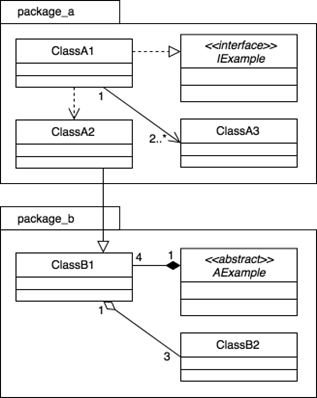
\includegraphics{Hinhve/Picture2.png}
%     \caption{Ví dụ thiết kế gói}
%     \label{fig:Fig2}
% \end{figure}

\subsubsection{Gói Client}
\label{subsubsection:systemdesign-package-client}
Hầu hết các gói trong \textbf{Client} đều tuân thủ theo mô hình MVVM, do đó các gói Views, ViewModels, HttpServices sẽ được thiết kế tương tự nhau. Để tránh lặp lại các biểu đồ, sau đây chỉ View (ProductListPage) sẽ làm mẫu cho các gói khác và được trình bày chi tiết trong hình \ref{fig:systemdesign-package-client-productlistpage}.
\begin{figure}[H]
    \centering
    \includegraphics[width=0.4\textwidth]{Hinhve/design/package/client/ProductListPage}
    \caption{Biểu đồ gói ListPage của Product}
    \label{fig:systemdesign-package-client-productlistpage}
\end{figure}
\textbf{View} chứa một lớp con \textbf{ViewModel} để xử lí logic và truyền tải dữ liệu giữa View và Model. Lớp \textbf{ViewModel} sẽ chứa các dữ liệu mà \textbf{View} của nó hiển thị, và khi người dùng thực hiện thao tác tới hệ thống, thì \textbf{ViewModel} sẽ dùng \textbf{HttpService} tương ứng để gọi API và cập nhật dữ liệu. Khi đó, \textbf{View} sẽ được cập nhật lại dữ liệu và hiển thị lên giao diện.
\vfill
\break

Hình \ref{fig:systemdesign-package-client-httpservices} mô tả các lớp hỗ trợ gọi API trong gói HttpServices.
\begin{figure}[H]
    \centering
    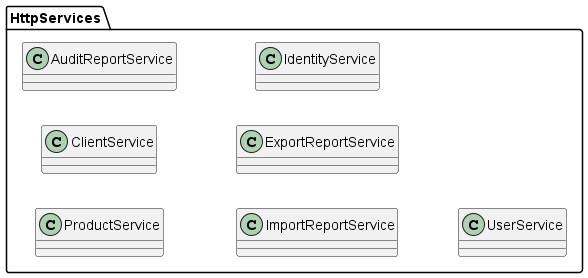
\includegraphics[width=0.9\textwidth]{Hinhve/design/package/client/HttpServices}
    \caption{Các biểu đồ gói HttpServices}
    \label{fig:systemdesign-package-client-httpservices}
\end{figure}

Hình \ref{fig:systemdesign-package-client-views} mô tả các lớp giao diện người dùng trong gói Views.
\begin{figure}[H]
    \centering
    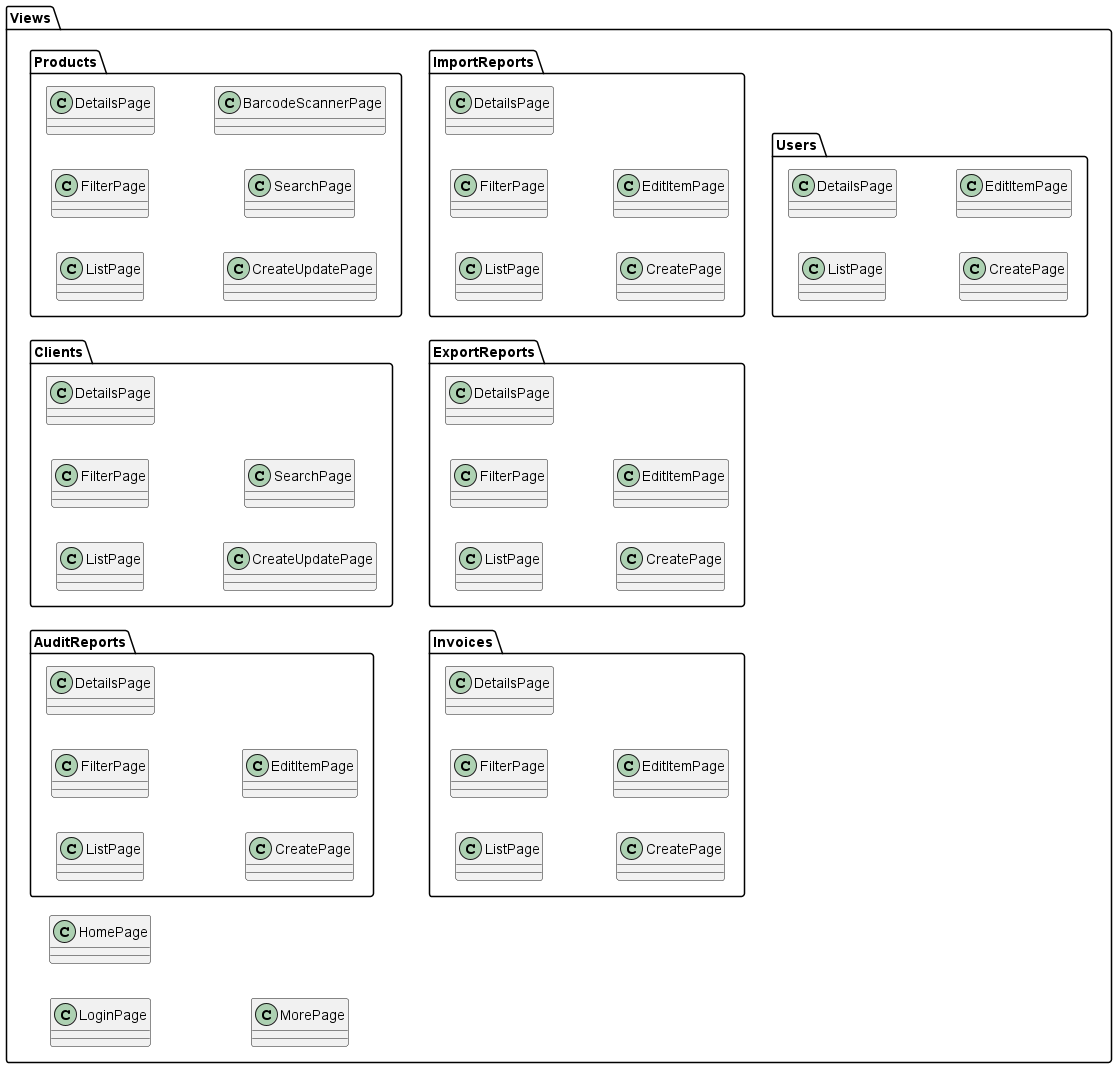
\includegraphics[width=1\textwidth]{Hinhve/design/package/client/Views}
    \caption{Các biểu đồ gói Views}
    \label{fig:systemdesign-package-client-views}
\end{figure}
\break

Hình \ref{fig:systemdesign-package-client-viewmodels} mô tả các lớp ViewModels.
\begin{figure}[H]
    \begin{subfigure}{\textwidth}
        \centering
        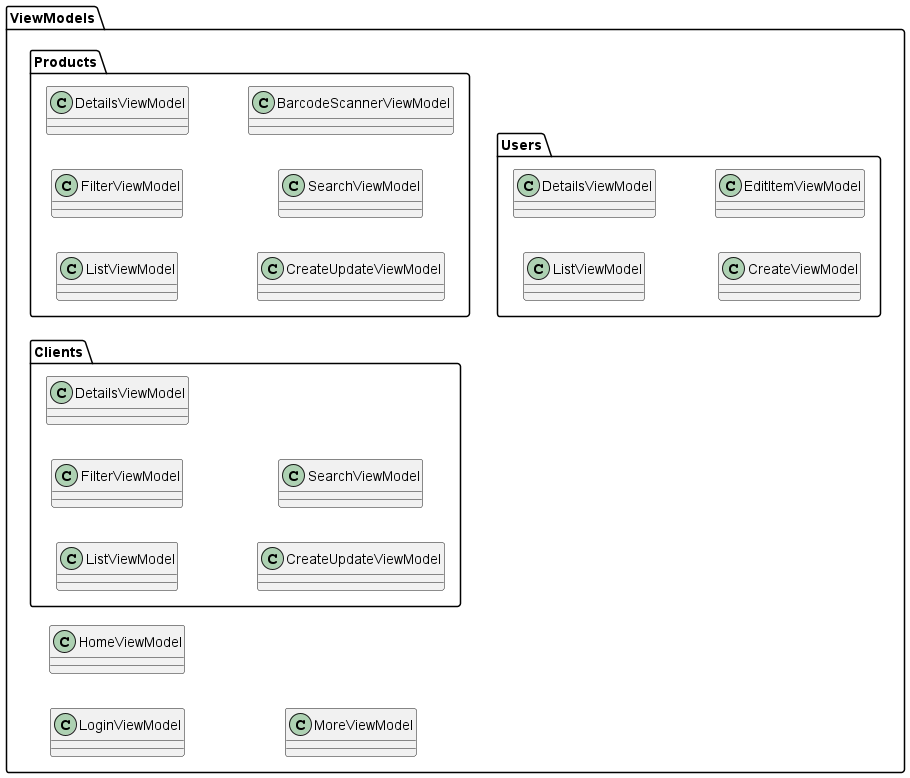
\includegraphics[width=1\linewidth]{Hinhve/design/package/client/ViewModels1}
    \end{subfigure}

    \begin{subfigure}{\textwidth}
        \centering
        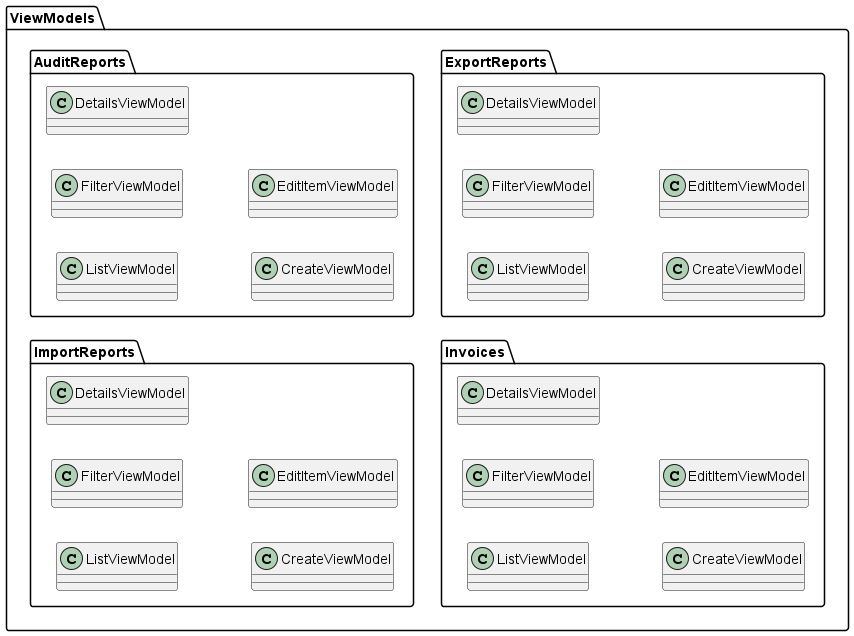
\includegraphics[width=0.9\linewidth]{Hinhve/design/package/client/ViewModels2}
    \end{subfigure}
    \caption{Các biểu đồ gói ViewModels}
    \label{fig:systemdesign-package-client-viewmodels}
\end{figure}
\vfill
\break


\subsubsection{Gói Server}
\label{subsubsection:systemdesign-package-server}
Áp dụng kiến trúc Clean Architecture, hầu hết tương ứng với mỗi thực thể thì sẽ luôn có một lớp kế thừa interface \textbf{IRepository} được định nghĩa trong tầng \textbf{Infrastructure}. Các lớp \textbf{Services} sẽ dùng các lớp đó để xử lí logic. Cuối cùng là lớp \textbf{Controller} sẽ định nghĩa các đầu API.

Ví dụ đối với thực thể \textit{Product}, các lớp liên quan tương tác với nhau sẽ được trình bày chi tiết trong hình \ref{fig:package-server-product}. Hình \ref{fig:package-server-domain} mô tả các thực thể của hệ thống.
\begin{figure}[H]
    \begin{subfigure}{0.59\textwidth}
        \centering
        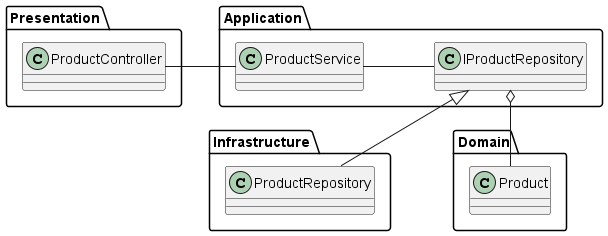
\includegraphics[width=1\linewidth]{Hinhve/design/package/server/Product}
        \caption{Biểu đồ các lớp liên quan tới sản phẩm}
        \label{fig:package-server-product}
    \end{subfigure}
    \begin{subfigure}{0.4\textwidth}
        \centering
        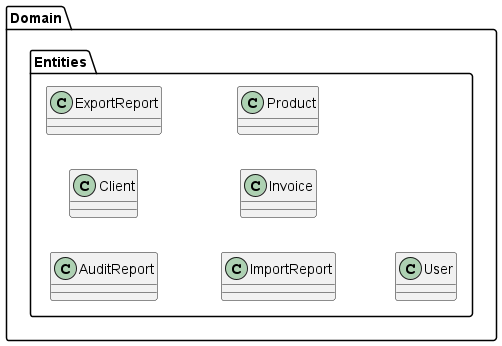
\includegraphics[width=1\linewidth]{Hinhve/design/package/server/Domain}
        \caption{Biểu đồ các lớp gói Domain}
        \label{fig:package-server-domain}
    \end{subfigure}
    \caption{Các biểu đồ gói Server}
    \label{fig:package-server}
\end{figure}

Hình \ref{fig:systemdesign-package-server-presentation} mô tả các lớp gói Presentation. Chúng chứa các đầu API để giao tiếp với thiết bị frontend.
\begin{figure}[H]
    \centering
    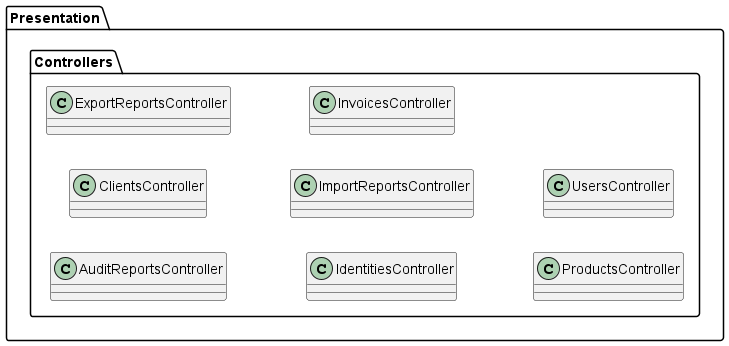
\includegraphics[width=1\textwidth]{Hinhve/design/package/server/Presentation}
    \caption{Biểu đồ gói Presentation}
    \label{fig:systemdesign-package-server-presentation}
\end{figure}
\break

Hình \ref{fig:systemdesign-package-server-application} mô tả các lớp gói Application.
\begin{figure}[H]
    \centering
    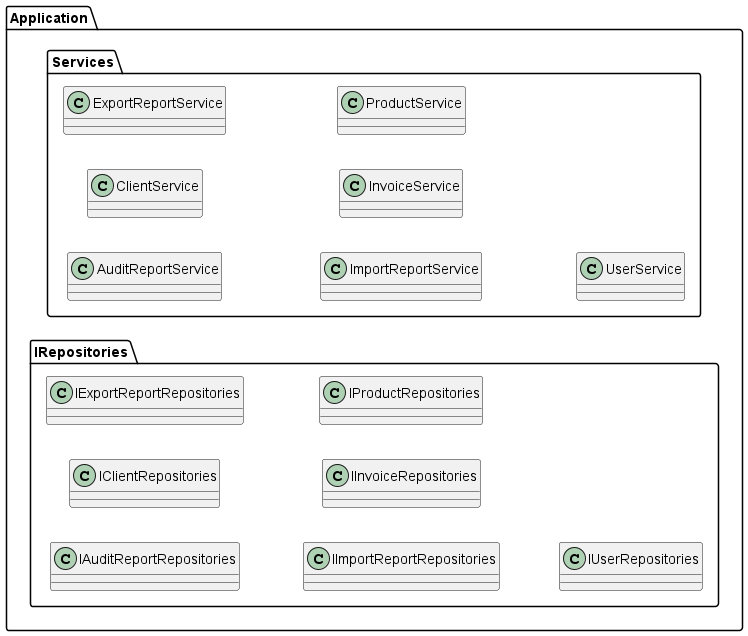
\includegraphics[width=1\textwidth]{Hinhve/design/package/server/Application}
    \caption{Biểu đồ gói Application}
    \label{fig:systemdesign-package-server-application}
\end{figure}

Hình \ref{fig:systemdesign-package-server-infrastructure} mô tả các lớp gói Infrastructure.
\begin{figure}[H]
    \centering
    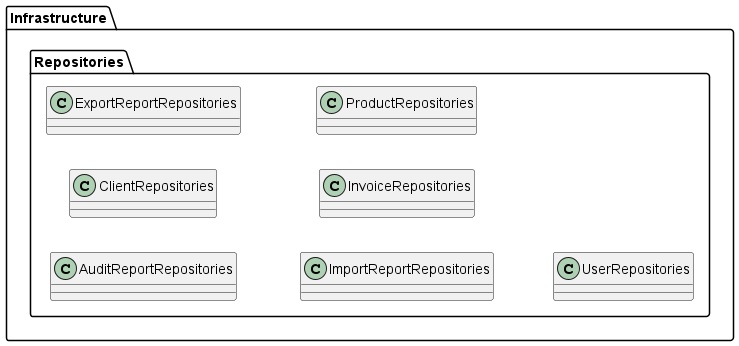
\includegraphics[width=1\textwidth]{Hinhve/design/package/server/Infrastructure}
    \caption{Biểu đồ gói Infrastructure}
    \label{fig:systemdesign-package-server-infrastructure}
\end{figure}
\break


\section{Thiết kế chi tiết}
\label{section:detaildesign}

\subsection{Thiết kế giao diện}
\label{subsection:detaildesign-ui}
% Phần này có độ dài từ hai đến ba trang. Sinh viên đặc tả thông tin về màn hình mà ứng dụng của mình hướng tới, bao gồm độ phân giải màn hình, kích thước màn hình, số lượng màu sắc hỗ trợ, v.v. Tiếp đến, sinh viên đưa ra các thống nhất/chuẩn hóa của mình khi thiết kế giao diện như thiết kế nút, điều khiển, vị trí hiển thị thông điệp phản hồi, phối màu, v.v. Sau cùng sinh viên đưa ra một số hình ảnh minh họa thiết kế giao diện cho các chức năng quan trọng nhất. Lưu ý, sinh viên không nhầm lẫn giao diện thiết kế với giao diện của sản phẩm sau cùng.
Bảng \ref{table:ui_standard} mô tả quy chuẩn thiết kế giao diện của hệ thống cho các màn hình và các thiết kế thành phần.
\begin{table}[H]
    \begin{tabularx}{\textwidth}{|l|X|}
        \hline
        Số lượng màu sắc hỗ trợ & 16 triệu màu         \\ \hline
        Font chữ sử dụng        & Open Sans            \\ \hline
        Màu nền chính           & \#FFFFFF (trắng)     \\ \hline
        Màu nền phụ             & \#F2F0F4 (xám nhạt)  \\ \hline
        Màu chữ chính           & \#000000 (đen)       \\ \hline
        Màu chữ phụ             & \#696969 (xám)       \\ \hline
        Màu cảnh báo            & \#FF5e52 (đỏ)        \\ \hline
        Màu thành công          & \#35A854 (xanh lá)   \\ \hline
        Màu thông tin           & \#247ECE (xanh biển) \\ \hline
        Ngôn ngữ hiển thị       & Tiếng Việt           \\ \hline
        Hỗ trợ chế độ màu tối   & Không                \\ \hline
        Vị trí thông báo lỗi    & Giữa màn hình        \\ \hline
        Múi giờ mặc định        & UTC+7                \\ \hline
    \end{tabularx}
    \caption{Quy chuẩn thiết kế giao diện}
    \label{table:ui_standard}
\end{table}


\subsection{Thiết kế lớp}
\label{subsection:detaildesign-class}
% Phần này có độ dài từ ba đến bốn trang. Sinh viên trình bày thiết kế chi tiết các thuộc tính và phương thức cho một số lớp chủ đạo/quan trọng nhất của ứng dụng (từ 2-4 lớp). Thiết kế chi tiết cho các lớp khác, nếu muốn trình bày, sinh viên đưa vào phần phụ lục.

% Để minh họa thiết kế lớp, sinh viên thiết kế luồng truyền thông điệp giữa các đối tượng tham gia cho 2 đến 3 use case quan trọng nào đó bằng biểu đồ trình tự (hoặc biểu đồ giao tiếp).
Để minh họa thiết kế lớp mà vẫn ngắn gọn súc tích, use case Quản lý phiếu nhập kho (được mô tả trong bảng use case \ref{table:uc-importreport-manage} và biểu đồ \ref{figure:sd-importreport-manage}) sẽ được chọn làm một ví dụ mẫu trong quá trình xử lí dữ liệu giữa các lớp với nhau. Sau đây là một số bảng thiết kế thuộc tính lớp, biểu đồ trình tự luồng truyền thông điệp giữa các đối tượng tham gia trong use case.

Bảng \ref{table:class-importreportcontroller} mô tả thiết kế lớp \textbf{ImportReportController} trong gói \textbf{Presentation}. Lớp này sẽ định nghĩa các đầu API để giao tiếp với thiết bị frontend.
\begin{table}[H]
    \begin{tabularx}{\textwidth}{|l|X|}
        \hline
        \multicolumn{2}{|c|}{\textbf{ImportReportController}}              \\ \hline
        \textbf{Tên thuộc tính}     & \textbf{Mô tả}                       \\ \hline
        ImportReportService service & Đối tượng để gọi các hàm xử lí logic \\ \hline
        \textbf{Tên hàm}            & \textbf{Mô tả}                       \\ \hline
        Get(string id)              & Lấy thông tin phiếu nhập kho bằng id \\ \hline
        Post(ImportReport entity)   & Tạo phiếu nhập kho                   \\ \hline
        Cancel(string id)           & Hủy phiếu nhập kho                   \\ \hline
        Delete(string id)           & Xóa phiếu nhập kho                   \\ \hline
    \end{tabularx}
    \caption{Bảng thiết kế lớp ImportReportController}
    \label{table:class-importreportcontroller}
\end{table}
\break

Bảng \ref{table:class-importreportservice} mô tả thiết kế lớp \textbf{ImportReportRepository} trong gói \textbf{Application}. Lớp này sẽ định nghĩa các hàm xử lí dữ liệu.
\begin{table}[H]
    \begin{tabularx}{\textwidth}{|l|X|}
        \hline
        \multicolumn{2}{|c|}{\textbf{ImportReportService}}                               \\ \hline
        \textbf{Tên thuộc tính}        & \textbf{Mô tả}                                  \\ \hline
        ImportReportRepository service & Đối tượng để gọi các hàm truy vấn cơ sở dữ liệu \\ \hline
        ProductRepository service      & Đối tượng để gọi các hàm truy vấn cơ sở dữ liệu \\ \hline
        \textbf{Tên hàm}               & \textbf{Mô tả}                                  \\ \hline
        Get(string id)                 & Lấy thông tin phiếu nhập kho bằng id            \\ \hline
        Create(ImportReport entity)    & Tạo phiếu nhập kho                              \\ \hline
        Cancel(string id)              & Hủy phiếu nhập kho                              \\ \hline
        Delete(string id)              & Xóa phiếu nhập kho                              \\ \hline
    \end{tabularx}
    \caption{Bảng thiết kế lớp ImportReportService}
    \label{table:class-importreportservice}
\end{table}

Bảng \ref{table:class-importreportrepository} mô tả thiết kế lớp \textbf{ImportReportRepository} trong gói \textbf{Infrastructure}. Lớp này sẽ định nghĩa các hàm truy vấn cơ sở dữ liệu.
\begin{table}[H]
    \begin{tabularx}{\textwidth}{|l|X|}
        \hline
        \multicolumn{2}{|c|}{\textbf{ImportReportRepository}}              \\ \hline
        \textbf{Tên thuộc tính}     & \textbf{Mô tả}                       \\ \hline
        MongoDatabase database      & Đối tượng kết nối cơ sở dữ liệu      \\ \hline
        \textbf{Tên hàm}            & \textbf{Mô tả}                       \\ \hline
        Get(string id)              & Lấy thông tin phiếu nhập kho bằng id \\ \hline
        Create(ImportReport entity) & Tạo phiếu nhập kho                   \\ \hline
        Update(string id, ...)      & Cập nhật phiếu nhập kho              \\ \hline
        Delete(string id)           & Xóa phiếu nhập kho                   \\ \hline
    \end{tabularx}
    \caption{Bảng thiết kế lớp ImportReportRepository}
    \label{table:class-importreportrepository}
\end{table}

Bảng \ref{table:class-productrepository} mô tả thiết kế lớp \textbf{ProductRepository} trong gói \textbf{Infrastructure}. Lớp này sẽ định nghĩa các hàm truy vấn cơ sở dữ liệu.
\begin{table}[H]
    \begin{tabularx}{\textwidth}{|l|X|}
        \hline
        \multicolumn{2}{|c|}{\textbf{ProductRepository}}                   \\ \hline
        \textbf{Tên thuộc tính} & \textbf{Mô tả}                           \\ \hline
        MongoDatabase database  & Đối tượng kết nối cơ sở dữ liệu          \\ \hline
        \textbf{Tên hàm}        & \textbf{Mô tả}                           \\ \hline
        Get(string id)          & Lấy thông tin sản phẩm bằng id           \\ \hline
        GetAll(string[] ids)    & Lấy thông tin nhiều sản phẩm bằng các id \\ \hline
        Create(Product entity)  & Tạo sản phẩm                             \\ \hline
        Update(string id, ...)  & Cập nhật sản phẩm                        \\ \hline
        Delete(string id)       & Xóa sản phẩm                             \\ \hline
    \end{tabularx}
    \caption{Bảng thiết kế lớp ProductRepository}
    \label{table:class-productrepository}
\end{table}
\break


Biểu đồ \ref{figure:sd-importreport-get} mô tả quá trình các thiết bị frontend gọi API để lấy thông tin phiếu nhập kho. Cụ thể, khi người dùng thực hiện thao tác lấy thông tin phiếu nhập kho, thì đối tượng \textbf{ImportReportController} sẽ nhận yêu cầu và gọi đến đối tượng \textbf{ImportReportService} để xử lí logic. Sau đó, \textbf{ImportReportService} sẽ gọi đến đối tượng \textbf{ImportReportRepository} để lấy thông tin từ cơ sở dữ liệu. Cuối cùng, \textbf{ImportReportRepository} sẽ trả về kết quả cho \textbf{ImportReportService}, \textbf{ImportReportService} sẽ trả về kết quả cho \textbf{ImportReportController}, \textbf{ImportReportController} sẽ trả về kết quả cho thiết bị frontend.
\begin{figure}[H]
    \centering
    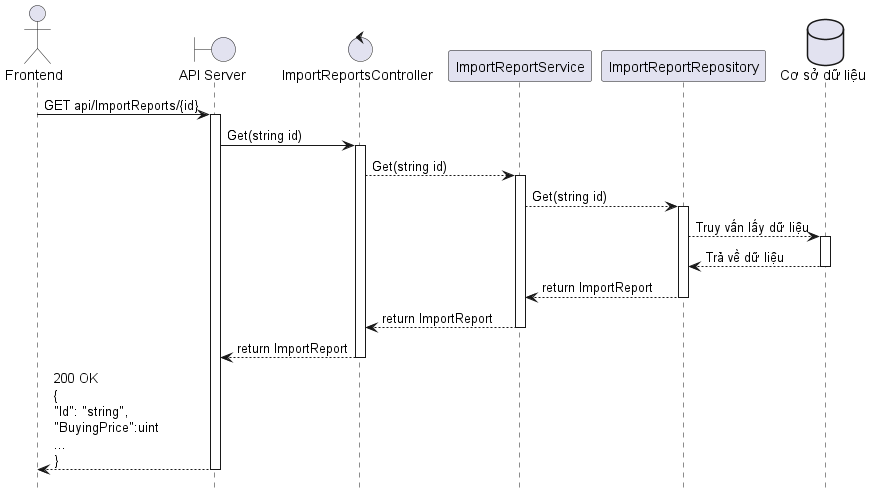
\includegraphics[width=1\textwidth]{Hinhve/design/class/ImportReportGETSequence}
    \caption{Biểu đồ trình tự Lấy thông tin phiếu nhập kho}
    \label{figure:sd-importreport-get}
\end{figure}

Biểu đồ \ref{figure:sd-importreport-patchcancel} mô tả quá trình thiết bị frontend gọi API để hủy phiếu nhập kho.
\begin{figure}[H]
    \centering
    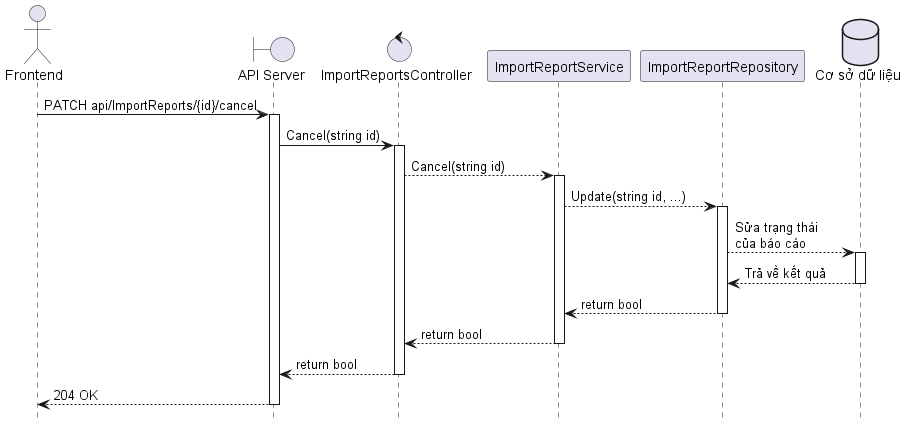
\includegraphics[width=1\textwidth]{Hinhve/design/class/ImportReportPATCHCancelSequence}
    \caption{Biểu đồ trình tự Hủy phiếu nhập kho}
    \label{figure:sd-importreport-patchcancel}
\end{figure}
\break

Biểu đồ \ref{figure:sd-importreport-post} mô tả quá trình thiết bị frontend gọi API để tạo phiếu nhập kho.
\begin{figure}[H]
    \centering
    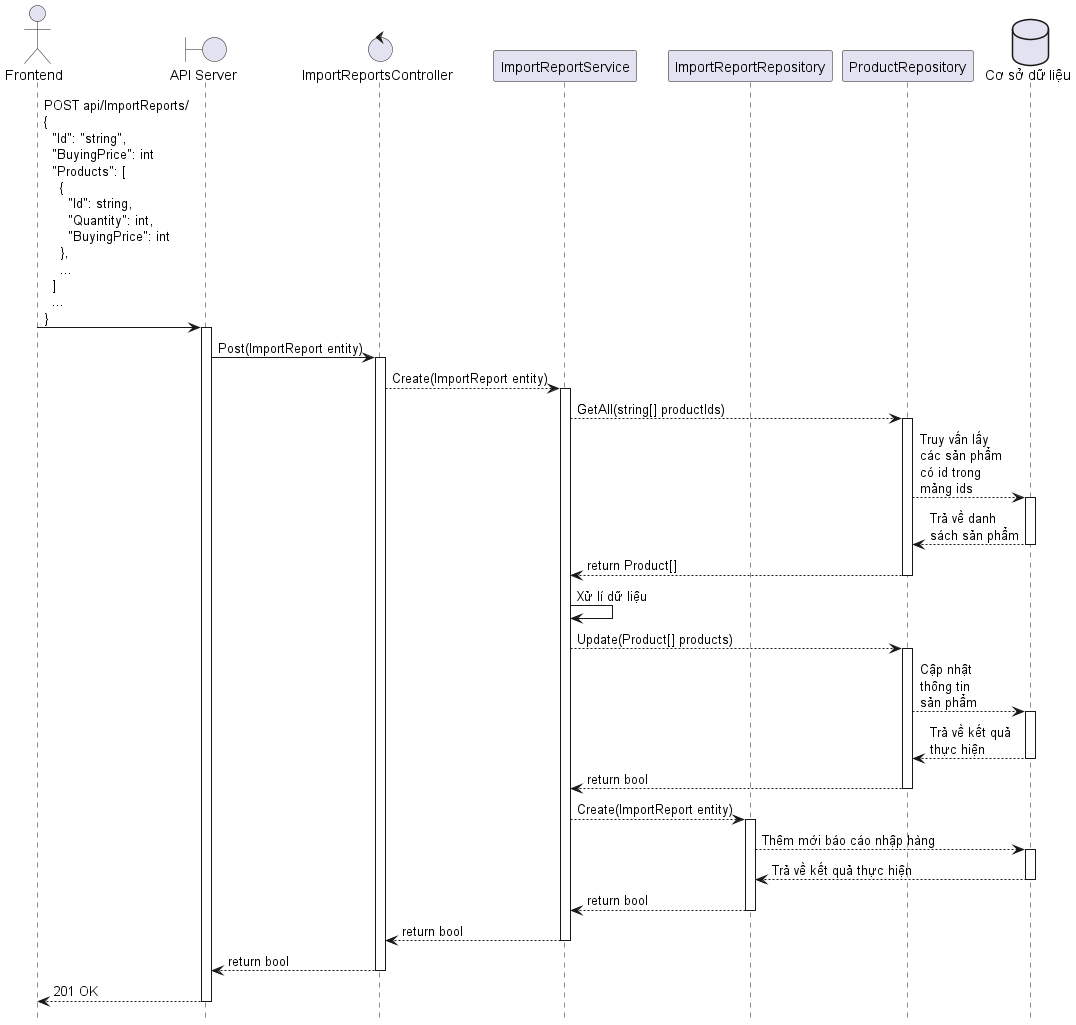
\includegraphics[width=1\textwidth]{Hinhve/design/class/ImportReportPOSTSequence}
    \caption{Biểu đồ trình tự Tạo phiếu nhập kho}
    \label{figure:sd-importreport-post}
\end{figure}

Biểu đồ \ref{figure:sd-importreport-delete} mô tả quá trình thiết bị frontend gọi API để xóa phiếu nhập kho.
\begin{figure}[H]
    \centering
    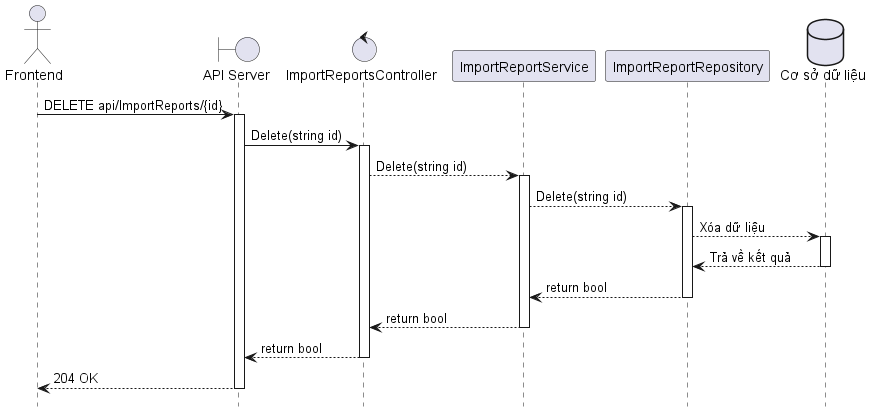
\includegraphics[width=0.9\textwidth]{Hinhve/design/class/ImportReportDELETESequence}
    \caption{Biểu đồ trình tự Xóa phiếu nhập kho}
    \label{figure:sd-importreport-delete}
\end{figure}
\break


\subsection{Thiết kế cơ sở dữ liệu}
\label{subsection:detaildesign-database}
% Phần này có độ dài từ hai đến bốn trang. Sinh viên thiết kế, vẽ và giải thích biểu đồ thực thể liên kết (E-R diagram). Từ đó, sinh viên thiết kế cơ sở dữ liệu tùy theo hệ quản trị cơ sở dữ liệu mà mình sử dụng (SQL, NoSQL, Firebase, v.v.)

\subsubsection{Biểu đồ thực thể liên kết}
\label{subsubsection:detaildesign-database-er}
Biểu đồ thực thể liên kết (E-R diagram) của hệ thống được trình bày trong hình \ref{fig:erdiagram}. Trong đó, các thực thể chính bao gồm: \textbf{User} (Người dùng), \textbf{Client} (Khách hàng), \textbf{Product} (Sản phẩm), \textbf{AuditReport} (Phiếu kiểm kho), \textbf{ImportReport} (Phiếu nhập kho), \textbf{ExportReport} (Phiếu xuất kho), \textbf{Invoice} (Hóa đơn).
\begin{figure}[H]
    \centering
    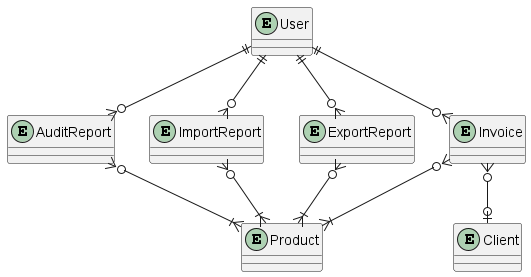
\includegraphics[width=1\textwidth]{Hinhve/design/class/EntityRelational}
    \caption{Biểu đồ thực thể liên kết}
    \label{fig:erdiagram}
\end{figure}
Các thực thể \textbf{AuditReport}, \textbf{ImportReport}, \textbf{ExportReport}, \textbf{Invoice} đều chứa một hoặc nhiều thực thể \textbf{Product} (ghi chép thay đổi hàng hóa), và chứa chính xác một thực thể \textbf{User} (người làm phiếu). Ngoài ra thực thể Invoice còn có thể chứa một thực thể \textbf{Client} (khách hàng mua hàng).
\vfill

\subsubsection{Chi tiết thực thể User}
\label{subsubsection:detaildesign-database-user}
Bảng \ref{table:database_user} là bảng cơ sở dữ liệu \textbf{User}, lưu trữ thông tin cá nhân người dùng. Cụ thể người dùng có thể là Quản lí, Nhân viên hay Quản trị viên.
\begin{table}[H]
    \centering
    \begin{tabularx}{\textwidth}{|p{4cm}|p{3cm}|X|}
        \hline
        \textbf{Tên trường} & \textbf{Kiểu dữ liệu} & \textbf{Mô tả} \\ \hline
        Id                  & string                & Mã định danh   \\ \hline
        Name                & string                & Tên người dùng \\ \hline
        Phonenumber         & string                & Số điện thoại  \\ \hline
        DateCreated         & DateTime              & Ngày tạo       \\ \hline
    \end{tabularx}
    \caption{Bảng cơ sở dữ liệu User}
    \label{table:database_user}
\end{table}
\break

Bảng \ref{table:database_userinfo} là bảng cơ sở dữ liệu \textbf{UserInfo}, lưu trữ thông tin vắn tắt của người dùng. Thực thể này được đính kèm vào các thực thể \textbf{AuditReport}, \textbf{ImportReport}, \textbf{ExportReport}, \textbf{Invoice}. Điều này giúp cho việc cho dù người dùng bị xóa khỏi hệ thống thì các phiếu vẫn có thể lưu trữ được thông tin người tạo phiếu đơn.
\begin{table}[H]
    \centering
    \begin{tabularx}{\textwidth}{|p{4cm}|p{3cm}|X|}
        \hline
        \textbf{Tên trường} & \textbf{Kiểu dữ liệu} & \textbf{Mô tả} \\ \hline
        Id                  & string                & Mã định danh   \\ \hline
        Name                & string                & Tên người dùng \\ \hline
    \end{tabularx}
    \caption{Bảng cơ sở dữ liệu UserInfo}
    \label{table:database_userinfo}
\end{table}


\subsubsection{Chi tiết thực thể Client}
\label{subsubsection:detaildesign-database-client}
Bảng \ref{table:database_client} là bảng cơ sở dữ liệu \textbf{Client}, lưu trữ thông tin cá nhân về khách hàng.
\begin{table}[H]
    \centering
    \begin{tabularx}{\textwidth}{|p{4cm}|p{3cm}|X|}
        \hline
        \textbf{Tên trường} & \textbf{Kiểu dữ liệu} & \textbf{Mô tả} \\ \hline
        Id                  & string                & Mã định danh   \\ \hline
        Name                & string                & Tên khách hàng \\ \hline
        Phonenumber         & string                & Số điện thoại  \\ \hline
        DateCreated         & DateTime              & Ngày tạo       \\ \hline
        Email               & string?               & Địa chỉ email  \\ \hline
        Address             & string?               & Địa chỉ        \\ \hline
        Description         & string?               & Mô tả          \\ \hline
    \end{tabularx}
    \caption{Bảng cơ sở dữ liệu Client}
    \label{table:database_client}
\end{table}

Bảng \ref{table:database_clientinfo} là bảng cơ sở dữ liệu \textbf{ClientInfo}, lưu trữ thông tin vắn tắt của khách hàng. Thực thể này được đính kèm vào thực thể \textbf{Invoice}. Điều này giúp cho việc cho dù khách hàng bị xóa khỏi hệ thống thì hóa đơn vẫn còn thông tin khách mua hàng.
\begin{table}[H]
    \centering
    \begin{tabularx}{\textwidth}{|p{4cm}|p{3cm}|X|}
        \hline
        \textbf{Tên trường} & \textbf{Kiểu dữ liệu} & \textbf{Mô tả} \\ \hline
        Id                  & string                & Mã định danh   \\ \hline
        Name                & string                & Tên khách hàng \\ \hline
        Phonenumber         & string                & Số điện thoại  \\ \hline
    \end{tabularx}
    \caption{Bảng cơ sở dữ liệu ClientInfo}
    \label{table:database_clientinfo}
\end{table}
\break


\subsubsection{Chi tiết thực thể Product}
\label{subsubsection:detaildesign-database-product}
Bảng \ref{table:database_product} là bảng cơ sở dữ liệu \textbf{Product}, lưu trữ thông tin về sản phẩm.
\begin{table}[H]
    \centering
    \begin{tabularx}{\textwidth}{|p{4cm}|p{3cm}|X|}
        \hline
        \textbf{Tên trường} & \textbf{Kiểu dữ liệu} & \textbf{Mô tả}   \\ \hline
        Id                  & string                & Mã định danh     \\ \hline
        Name                & string                & Tên sản phẩm     \\ \hline
        Barcode             & string                & Mã vạch          \\ \hline
        Group               & string?               & Nhóm sản phẩm    \\ \hline
        Brand               & string?               & Thương hiệu      \\ \hline
        StoragePosition     & string?               & Vị trí lưu trữ   \\ \hline
        Description         & string?               & Mô tả            \\ \hline
        BuyingPrice         & uint                  & Giá nhập         \\ \hline
        SellingPrice        & uint                  & Giá bán          \\ \hline
        InStock             & uint                  & Số lượng tồn kho \\ \hline
        DateCreated         & DateTime              & Ngày tạo         \\ \hline
    \end{tabularx}
    \caption{Bảng cơ sở dữ liệu Product}
    \label{table:database_product}
\end{table}


\subsubsection{Chi tiết thực thể AuditReport}
\label{subsubsection:detaildesign-database-auditreport}
Bảng \ref{table:database_auditreport} là bảng cơ sở dữ liệu \textbf{AuditReport}, lưu trữ thông tin phiếu kiểm kho.
\begin{table}[H]
    \centering
    \begin{tabularx}{\textwidth}{|p{4cm}|p{3cm}|X|}
        \hline
        \textbf{Tên trường} & \textbf{Kiểu dữ liệu}                              & \textbf{Mô tả}            \\ \hline
        Id                  & string                                             & Mã định danh              \\ \hline
        Author              & UserInfo                                           & Thông tin người tạo phiếu \\
                            & (bảng \ref{table:database_userinfo})               &                           \\ \hline
        DateCreated         & DateTime                                           & Ngày tạo                  \\ \hline
        DateDeleted         & DateTime?                                          & Ngày xóa                  \\ \hline
        ProductItems        & List<ARPI>                                         & Danh sách sản phẩm        \\
                            & (bảng \ref{table:database_auditreportproductitem}) &                           \\ \hline
    \end{tabularx}
    \caption{Bảng cơ sở dữ liệu AuditReport}
    \label{table:database_auditreport}
\end{table}

Bảng \ref{table:database_auditreportproductitem} là bảng cơ sở dữ liệu \textbf{AuditReportProductItem}, lưu trữ thông tin chi tiết về các sản phẩm trong phiếu kiểm kho.
\begin{table}[H]
    \centering
    \begin{tabularx}{\textwidth}{|p{4cm}|p{3cm}|X|}
        \hline
        \textbf{Tên trường} & \textbf{Kiểu dữ liệu} & \textbf{Mô tả}         \\ \hline
        Id                  & string                & Mã sản phẩm            \\ \hline
        Name                & string                & Tên sản phẩm           \\ \hline
        Barcode             & string                & Mã vạch                \\ \hline
        OriginalQuantity    & uint                  & Số lượng ban đầu       \\ \hline
        AdjustedQuantity    & uint                  & Số lượng đã điều chỉnh \\ \hline
    \end{tabularx}
    \caption{Bảng cơ sở dữ liệu AuditReportProductItem}
    \label{table:database_auditreportproductitem}
\end{table}
\break


\subsubsection{Chi tiết thực thể ExportReport}
\label{subsubsection:detaildesign-database-exportreport}
Bảng \ref{table:database_exportreport} mô tả bảng cơ sở dữ liệu \textbf{ExportReport} của phiếu xuất kho.
\begin{table}[H]
    \centering
    \begin{tabularx}{\textwidth}{|p{4cm}|p{3cm}|X|}
        \hline
        \textbf{Tên trường} & \textbf{Kiểu dữ liệu}                               & \textbf{Mô tả}            \\ \hline
        Id                  & string                                              & Mã định danh              \\ \hline
        Author              & UserInfo                                            & Thông tin người tạo phiếu \\
                            & (bảng \ref{table:database_userinfo})                &                           \\ \hline
        InvoiceId           & string?                                             & Mã hóa đơn                \\ \hline
        DateCreated         & DateTime                                            & Ngày tạo                  \\ \hline
        DateCancelled       & DateTime?                                           & Ngày hủy                  \\ \hline
        DateDeleted         & DateTime?                                           & Ngày xóa                  \\ \hline
        ProductItems        & List<ERPI>                                          & Danh sách sản phẩm        \\
                            & (bảng \ref{table:database_exportreportproductitem}) &                           \\ \hline
    \end{tabularx}
    \caption{Bảng cơ sở dữ liệu ExportReport}
    \label{table:database_exportreport}
\end{table}

Bảng \ref{table:database_exportreportproductitem} mô tả bảng cơ sở dữ liệu \textbf{ExportReportProductItem}, lưu trữ thông tin chi tiết về các sản phẩm trong phiếu xuất kho. Cho dù sản phẩm bị xóa khỏi hệ thống thì phiếu xuất kho vẫn còn thông tin.
\begin{table}[H]
    \centering
    \begin{tabularx}{\textwidth}{|p{4cm}|p{3cm}|X|}
        \hline
        \textbf{Tên trường} & \textbf{Kiểu dữ liệu} & \textbf{Mô tả} \\ \hline
        Id                  & string                & Mã sản phẩm    \\ \hline
        Name                & string                & Tên sản phẩm   \\ \hline
        Barcode             & string                & Mã vạch        \\ \hline
        Quantity            & uint                  & Số lượng       \\ \hline
    \end{tabularx}
    \caption{Bảng cơ sở dữ liệu ExportReportProductItem}
    \label{table:database_exportreportproductitem}
\end{table}


\subsubsection{Chi tiết thực thể ImportReport}
\label{subsubsection:detaildesign-database-importreport}
Bảng \ref{table:database_importreport} là bảng cơ sở dữ liệu \textbf{ImportReport}, lưu thông tin phiếu nhập kho.
\begin{table}[H]
    \centering
    \begin{tabularx}{\textwidth}{|p{4cm}|p{3cm}|X|}
        \hline
        \textbf{Tên trường} & \textbf{Kiểu dữ liệu}                               & \textbf{Mô tả}            \\ \hline
        Id                  & string                                              & Mã định danh              \\ \hline
        Author              & UserInfo                                            & Thông tin người tạo phiếu \\
                            & (bảng \ref{table:database_userinfo})                &                           \\ \hline
        DateCreated         & DateTime                                            & Ngày tạo                  \\ \hline
        DateCancelled       & DateTime?                                           & Ngày hủy                  \\ \hline
        DateDeleted         & DateTime?                                           & Ngày xóa                  \\ \hline
        ProductItems        & List<IRPI>                                          & Danh sách sản phẩm        \\
                            & (bảng \ref{table:database_importreportproductitem}) &                           \\ \hline
    \end{tabularx}
    \caption{Bảng cơ sở dữ liệu ImportReport}
    \label{table:database_importreport}
\end{table}
\break

Bảng \ref{table:database_importreportproductitem} là bảng cơ sở dữ liệu \textbf{ImportReportProductItem}, lưu trữ thông tin chi tiết về các sản phẩm trong phiếu nhập kho.
\begin{table}[H]
    \centering
    \begin{tabularx}{\textwidth}{|p{4cm}|p{3cm}|X|}
        \hline
        \textbf{Tên trường} & \textbf{Kiểu dữ liệu} & \textbf{Mô tả} \\ \hline
        Id                  & string                & Mã sản phẩm    \\ \hline
        Name                & string                & Tên sản phẩm   \\ \hline
        Barcode             & string                & Mã vạch        \\ \hline
        Quantity            & uint                  & Số lượng       \\ \hline
        Price               & uint                  & Giá nhập       \\ \hline
    \end{tabularx}
    \caption{Bảng cơ sở dữ liệu ImportReportProductItem}
    \label{table:database_importreportproductitem}
\end{table}


\subsubsection{Chi tiết thực thể Invoice}
\label{subsubsection:detaildesign-database-invoice}
Bảng \ref{table:database_invoice} là bảng cơ sở dữ liệu \textbf{Invoice}, lưu trữ thông tin hóa đơn.
\begin{table}[H]
    \centering
    \begin{tabularx}{\textwidth}{|p{4cm}|p{3cm}|X|}
        \hline
        \textbf{Tên trường} & \textbf{Kiểu dữ liệu}                          & \textbf{Mô tả}            \\ \hline
        Id                  & string                                         & Mã định danh              \\ \hline
        Author              & UserInfo                                       & Thông tin người tạo phiếu \\
                            & (bảng \ref{table:database_userinfo})           &                           \\ \hline
        Client              & ClientInfo                                     & Thông tin khách hàng      \\
                            & (bảng \ref{table:database_clientinfo})         &                           \\ \hline
        ExportReportId      & string                                         & Mã phiếu xuất kho         \\ \hline
        GrandTotal          & uint                                           & Thành tiền                \\ \hline
        DateCreated         & DateTime                                       & Ngày tạo                  \\ \hline
        DatePaid            & DateTime?                                      & Ngày thanh toán           \\ \hline
        DateCancelled       & DateTime?                                      & Ngày hủy                  \\ \hline
        DateDeleted         & DateTime?                                      & Ngày xóa                  \\ \hline
        ProductItems        & List<IPI>                                      & Danh sách sản phẩm        \\
                            & (bảng \ref{table:database_invoiceproductitem}) &                           \\ \hline
    \end{tabularx}
    \caption{Bảng cơ sở dữ liệu Invoice}
    \label{table:database_invoice}
\end{table}

Bảng \ref{table:database_invoiceproductitem} là bảng cơ sở dữ liệu \textbf{InvoiceProductItem}, lưu trữ thông tin chi tiết về các sản phẩm trong hóa đơn.
\begin{table}[H]
    \centering
    \begin{tabularx}{\textwidth}{|p{4cm}|p{3cm}|X|}
        \hline
        \textbf{Tên trường} & \textbf{Kiểu dữ liệu} & \textbf{Mô tả} \\ \hline
        Id                  & string                & Mã sản phẩm    \\ \hline
        Name                & string                & Tên sản phẩm   \\ \hline
        Barcode             & string                & Mã vạch        \\ \hline
        Quantity            & uint                  & Số lượng       \\ \hline
        Price               & uint                  & Giá bán        \\ \hline
    \end{tabularx}
    \caption{Bảng cơ sở dữ liệu InvoiceProductItem}
    \label{table:database_invoiceproductitem}
\end{table}
\break


\section{Xây dựng ứng dụng}
\label{section:implementation}

\subsection{Thư viện và công cụ sử dụng}
\label{subsection:implementation-toolkit}
% Sinh viên liệt kê các công cụ, ngôn ngữ lập trình, API, thư viện, IDE, công cụ kiểm thử, v.v. mà mình sử dụng để phát triển ứng dụng. Mỗi công cụ phải được chỉ rõ phiên bản sử dụng. SV nên kẻ bảng mô tả tương tự như Bảng \ref{table:my_label}. Nếu có nhiều nội dung trình bày, sinh viên cần xoay ngang bảng.

% \begin{table}[H]
%     \centering{}
%     \begin{tabular}{lll}
%         \hline
%         \textbf{Mục đích} & \textbf{Công cụ}       & \textbf{Địa chỉ URL}    \\ \hline
%         IDE lập trình     & Eclipse Oxygen a64 bit & http://www.eclipse.org/ \\ \hline
%         v.v.              & v.v.                   & v.v.                    \\ \hline
%     \end{tabular}
%     \caption{Danh sách thư viện và công cụ sử dụng}
%     \label{fig:my_label}
% \end{table}
\begin{table}[H]
    \centering
    \begin{tabularx}{\textwidth}{|X|X|c|}
        \hline
        \textbf{Công cụ}     & \textbf{Mục đích}     & \textbf{Địa chỉ URL}                                                                             \\ \hline
        Visual Studio Code   & IDE lập trình         & \href{https://code.visualstudio.com/}{\color{blue}\underline{Link}}                              \\ \hline
        Visual Studio 2022   & IDE lập trình         & \href{https://visualstudio.microsoft.com/}{\color{blue}\underline{Link}}                         \\ \hline
        C\#                  & Ngôn ngữ lập trình    & \href{https://docs.microsoft.com/en-us/dotnet/csharp/}{\color{blue}\underline{Link}}             \\ \hline
        .NET 7.0             & Framework             & \href{https://dotnet.microsoft.com/}{\color{blue}\underline{Link}}                               \\ \hline
        .ASP.NET Core 7.0    & API Framework         & \href{https://dotnet.microsoft.com/en-us/apps/aspnet/}{\color{blue}\underline{Link}}             \\ \hline
        .NET MAUI            & UI Framework          & \href{https://docs.microsoft.com/en-us/dotnet/maui/}{\color{blue}\underline{Link}}               \\ \hline
        MongoDB              & Cơ sở dữ liệu         & \href{https://www.mongodb.com/}{\color{blue}\underline{Link}}                                    \\ \hline
        BarcodeScanning.MAUI & Thư viện quét mã vạch & \href{https://www.nuget.org/packages/BarcodeScanning.Native.Maui/}{\color{blue}\underline{Link}} \\ \hline
        PlantUML             & Vẽ biểu đồ            & \href{https://plantuml.com/}{\color{blue}\underline{Link}}                                       \\ \hline
        Docker               & Công cụ Deploy        & \href{https://www.docker.com/}{\color{blue}\underline{Link}}                                     \\ \hline
    \end{tabularx}
    \caption{Danh sách thư viện và công cụ sử dụng}
    \label{table:implementation_toolkit}
\end{table}


\subsection{Kết quả đạt được}
% Sinh viên trước tiên mô tả kết quả đạt được của mình là gì, ví dụ như các sản phẩm được đóng gói là gì, bao gồm những thành phần nào, ý nghĩa, vai trò?

% Sinh viên cần thống kê các thông tin về ứng dụng của mình như: số dòng code, số lớp, số gói, dung lượng toàn bộ mã nguồn, dung lượng của từng sản phẩm đóng gói, v.v. Tương tự như phần liệt kê về công cụ sử dụng, sinh viên cũng nên dùng bảng để mô tả phần thông tin thống kê này.
Dự án đã được đóng gói thành hai sản phẩm: ứng dụng di động và ứng dụng server. Ứng dụng di động được đóng gói thành file APK, có thể cài đặt trên các thiết bị chạy hệ điều hành Android. Ứng dụng server được đóng gói thành Docker Compose file, có thể triển khai trên các máy chủ đã cài đặt Docker. Các sản phẩm đã hoàn thiện đầy đủ các chức năng được đề xuất.

Ứng dụng Server có các thành phần chính như sau:
\begin{itemize}
    \item \textbf{API}: API server, cung cấp các API để ứng dụng di động gọi.
    \item \textbf{Database}: Cơ sở dữ liệu MongoDB.
\end{itemize}

Ứng dụng di động có các thành phần chính như sau:
\begin{itemize}
    \item \textbf{MAUI App}: Ứng dụng di động, cung cấp giao diện người dùng.
\end{itemize}

Bảng \ref{table:implementation-statistics} là bảng thống kê về ứng dụng Server và ứng dụng di động.
\begin{table}[H]
    \begin{tabularx}{\textwidth}{|l|X|}
        \hline
        \textbf{Tiêu chí}           & \textbf{Thông số} \\ \hline
        Số dòng code                & 16,030 dòng       \\ \hline
        Số lớp                      & 106 lớp           \\ \hline
        Số gói                      & 12 gói            \\ \hline
        Dung lượng mã nguồn         & 12.9 MB           \\ \hline
        Dung lượng ứng dụng Android & 35 MB             \\ \hline
    \end{tabularx}
    \caption{Thông tin thống kê}
    \label{table:implementation-statistics}
\end{table}
\break


\subsection{Minh họa các chức năng chính}
% Sinh viên lựa chọn và đưa ra màn hình cho các chức năng chính, quan trọng, và thú vị nhất. Mỗi giao diện cần phải có lời giải thích ngắn gọn. Khi giải thích, sinh viên có thể kết hợp với các chú thích ở trong hình ảnh giao diện.
Để minh họa cho sản phẩm cuối của hệ thống và giữ cho đề mục ngắn gọn, sau đây là các màn hình cho một số chức năng chính tiêu biểu, được chụp từ ứng dụng di động trên hệ điều hành Android.

\subsubsection{Chức năng hóa đơn}
Hình \ref{figure:screen-invoicelistpage} là màn hình danh sách hóa đơn. Tại đây người dùng có thể xem danh sách hóa đơn đã tạo, và có thể tạo hóa đơn mới bằng cách nhấn vào nút " + " ở góc phải màn hình. Người dùng có thể lọc danh sách hóa đơn bằng cách nhấn vào nút hình kính lúp để hiện màn hình bộ lọc. Hình \ref{figure:screen-invoicefilterpage} là màn hình bộ lọc hóa đơn. Tại đây người dùng có thể lọc danh sách hóa đơn theo các trường tên sản phẩm, tên khách hàng, tên người bán, ngày tạo, và theo trạng thái hóa đơn.
\begin{figure}[H]
    \begin{subfigure}{0.49\linewidth}
        \centering
        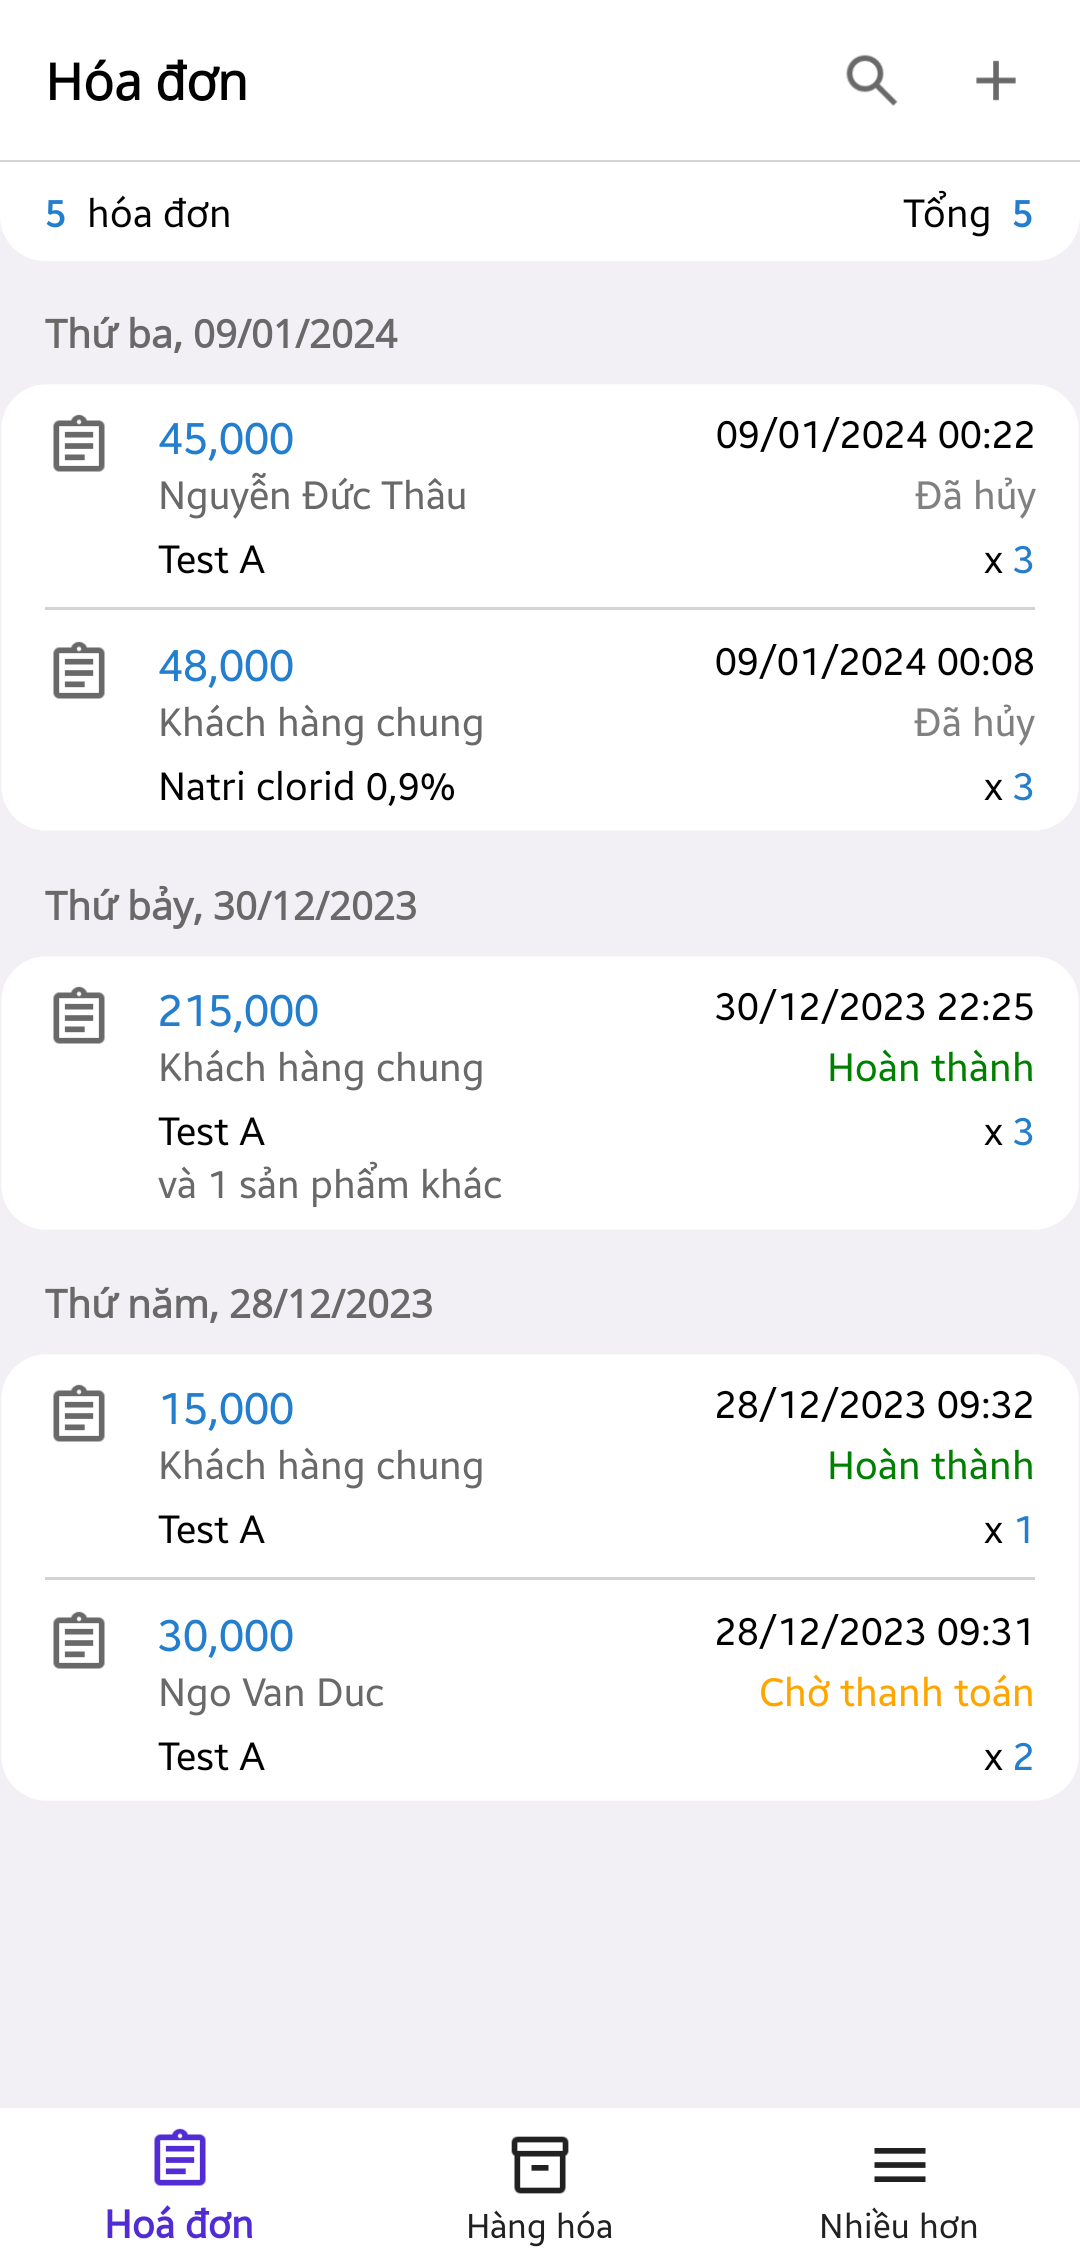
\includegraphics[width=0.9\linewidth]{Hinhve/design/screens/InvoiceListPage}
        \caption{Màn hình danh sách hóa đơn}
        \label{figure:screen-invoicelistpage}
    \end{subfigure}
    \begin{subfigure}{0.5\linewidth}
        \centering
        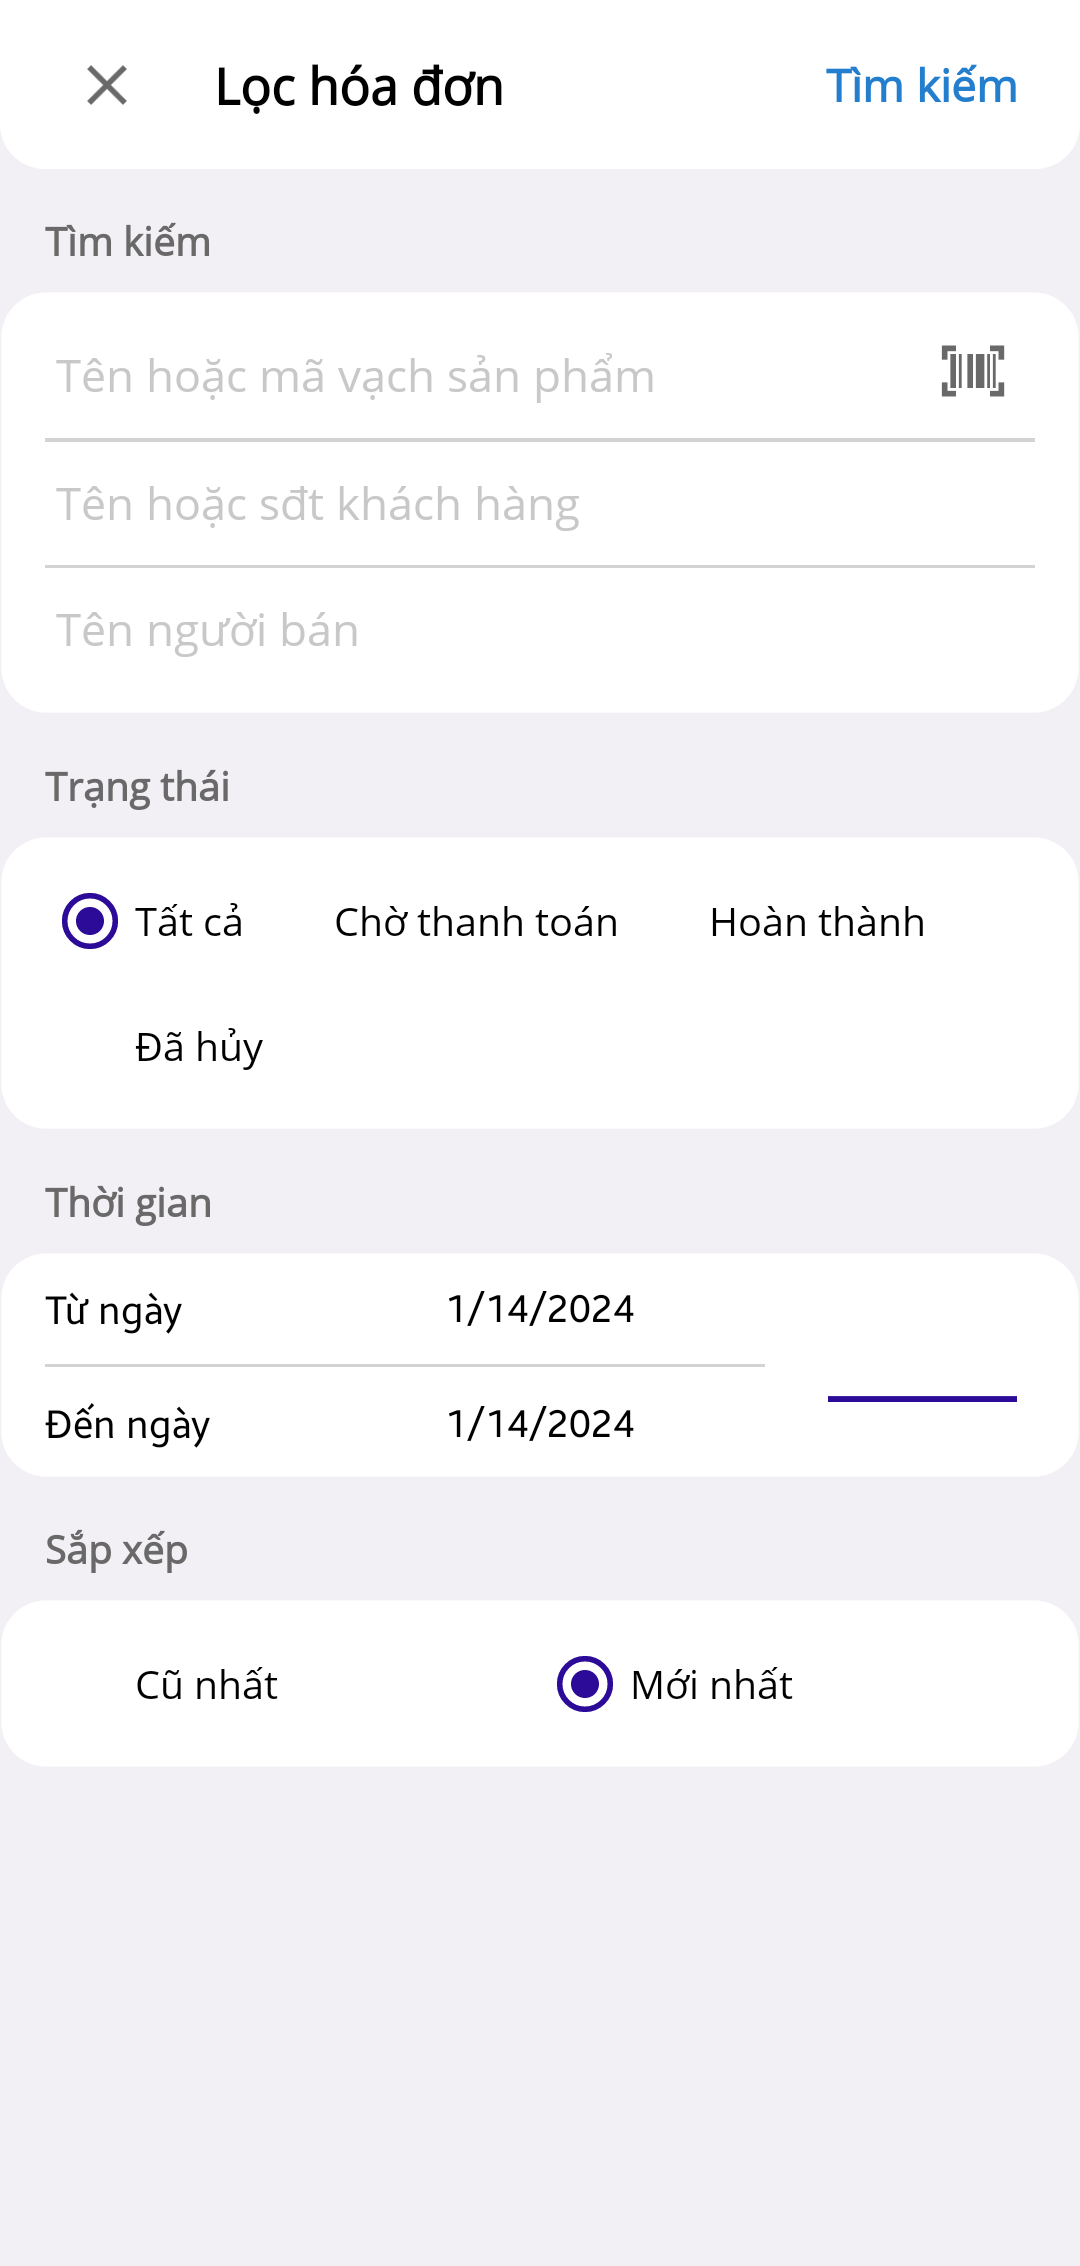
\includegraphics[width=0.9\linewidth]{Hinhve/design/screens/InvoiceFilterPage}
        \caption{Màn hình lọc hóa đơn}
        \label{figure:screen-invoicefilterpage}
    \end{subfigure}
    \caption{Các màn hình hóa đơn}
    \label{figure:screen-invoicepages1}
\end{figure}
\break

Hình \ref{figure:screen-invoicecreatepage} là màn hình tạo mới hóa đơn. Tại đây người dùng có thể thêm sản phẩm vào hóa đơn bằng cách nhấn vào nút " + Thêm ". Thêm nữa, người dùng có thể chọn khách hàng đã lưu trong hệ thống từ trước vào hóa đơn bằng cách nhấn vào thanh " Khách hàng ". Sau đó, mục thành tiền sẽ là giá tiền hóa đơn có thể thay đổi tùy vào người bán hàng. Mặc định hóa đơn sẽ có trạng thái "Chưa thanh toán", để thay đổi, người dùng có thể tích vào ô " Đã thanh toán ". Ngoài ra, để xóa sản phẩm khỏi hóa đơn, người dùng có thể vuốt sang trái sản phẩm hay vuốt sang phải để xem chi tiết hơn sản phẩm đó.

Hình \ref{figure:screen-invoicedetailspage} là màn hình chi tiết hóa đơn. Ở đây chứa mọi thông tin chi tiết về hóa đơn, hơn nữa người dùng có thể hủy hay xóa hóa đơn, và có thể thanh toán hóa đơn. Mọi chức năng đó có thể thực hiện bằng cách nhấn vào nút " \vdots{} " ở góc phải màn hình.
\begin{figure}[H]
    \begin{subfigure}{0.49\linewidth}
        \centering
        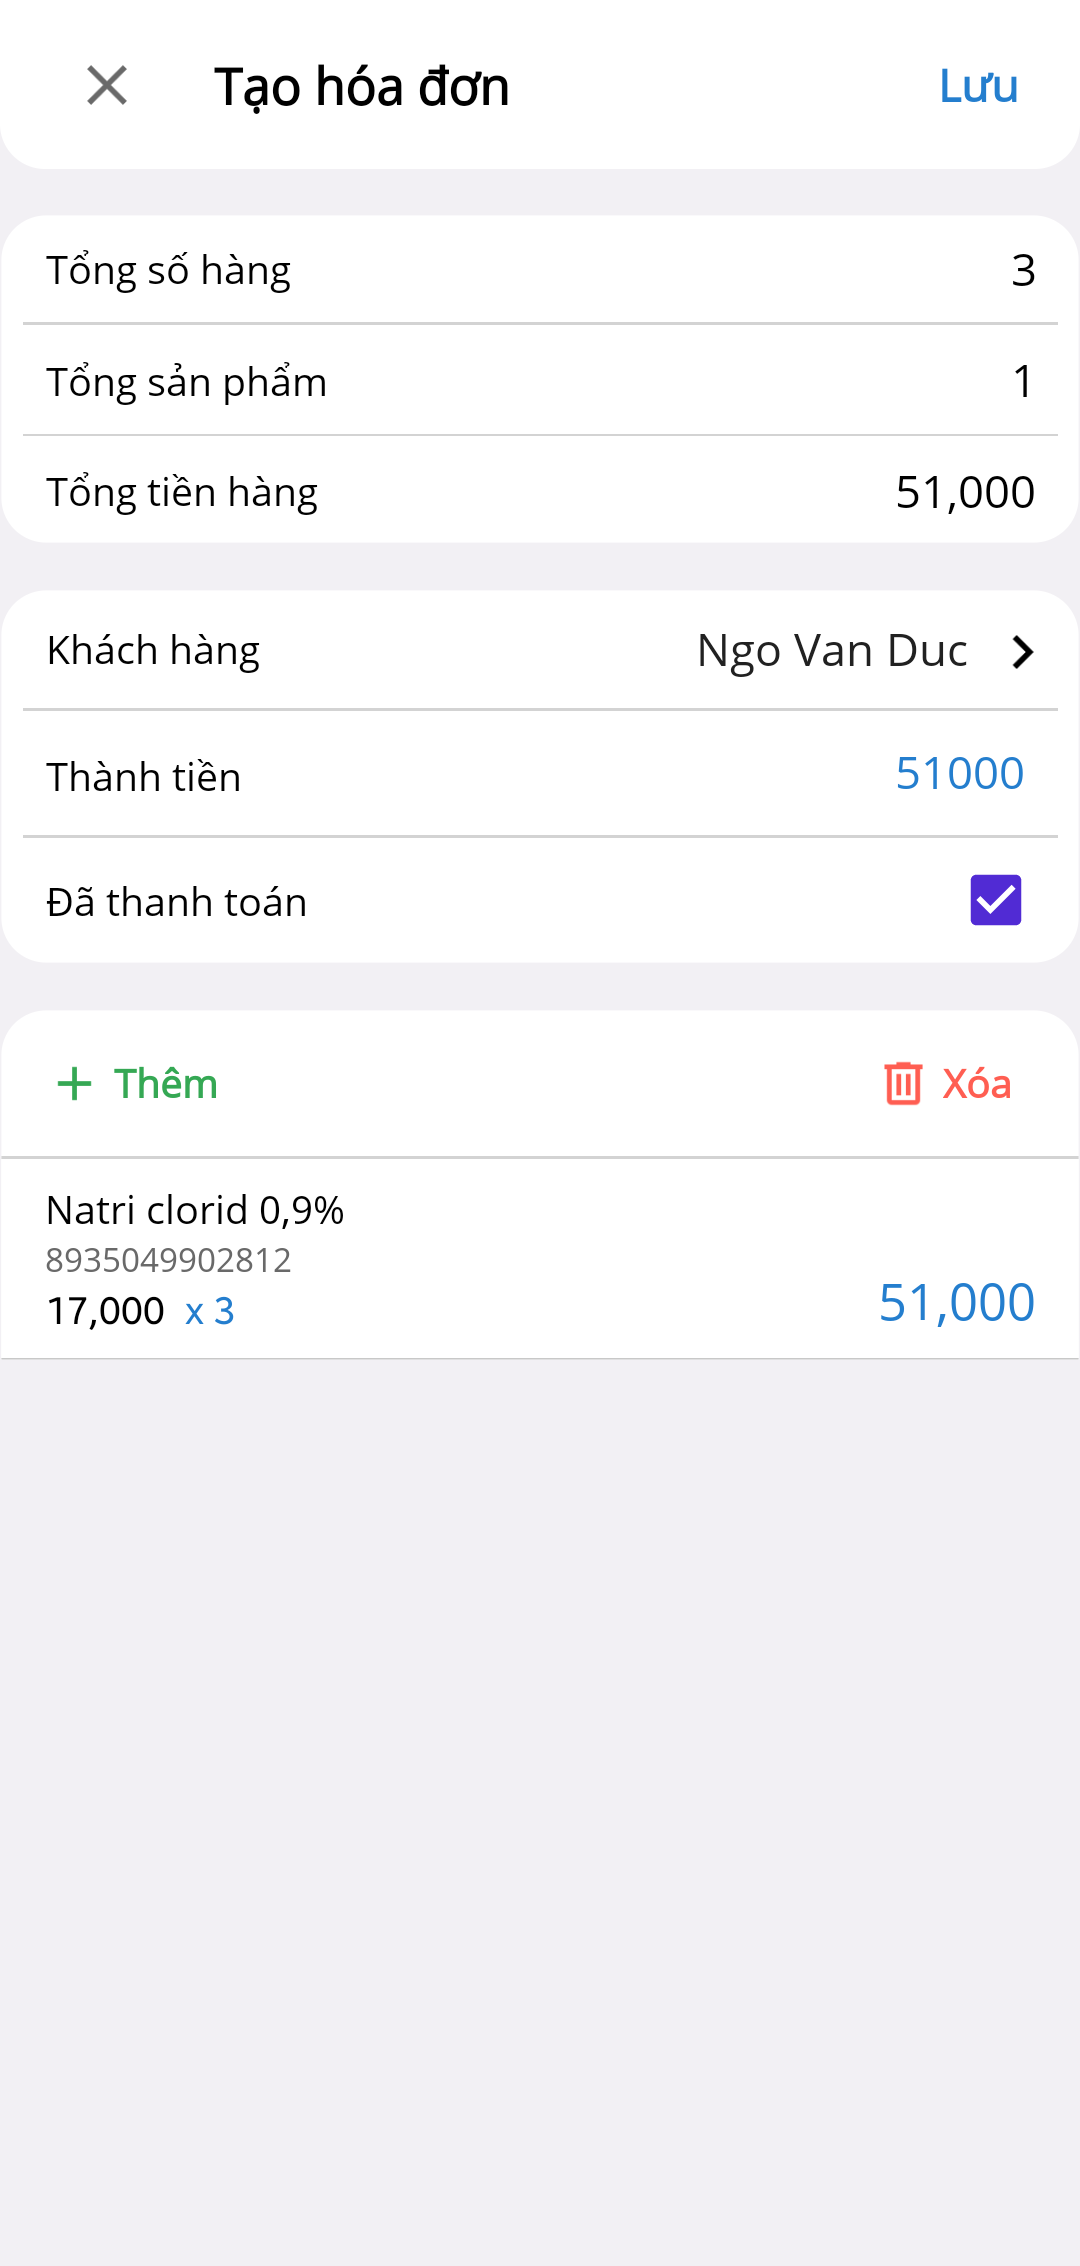
\includegraphics[width=0.9\linewidth]{Hinhve/design/screens/InvoiceCreatePage}
        \caption{Màn hình tạo mới hóa đơn}
        \label{figure:screen-invoicecreatepage}
    \end{subfigure}
    \begin{subfigure}{0.5\linewidth}
        \centering
        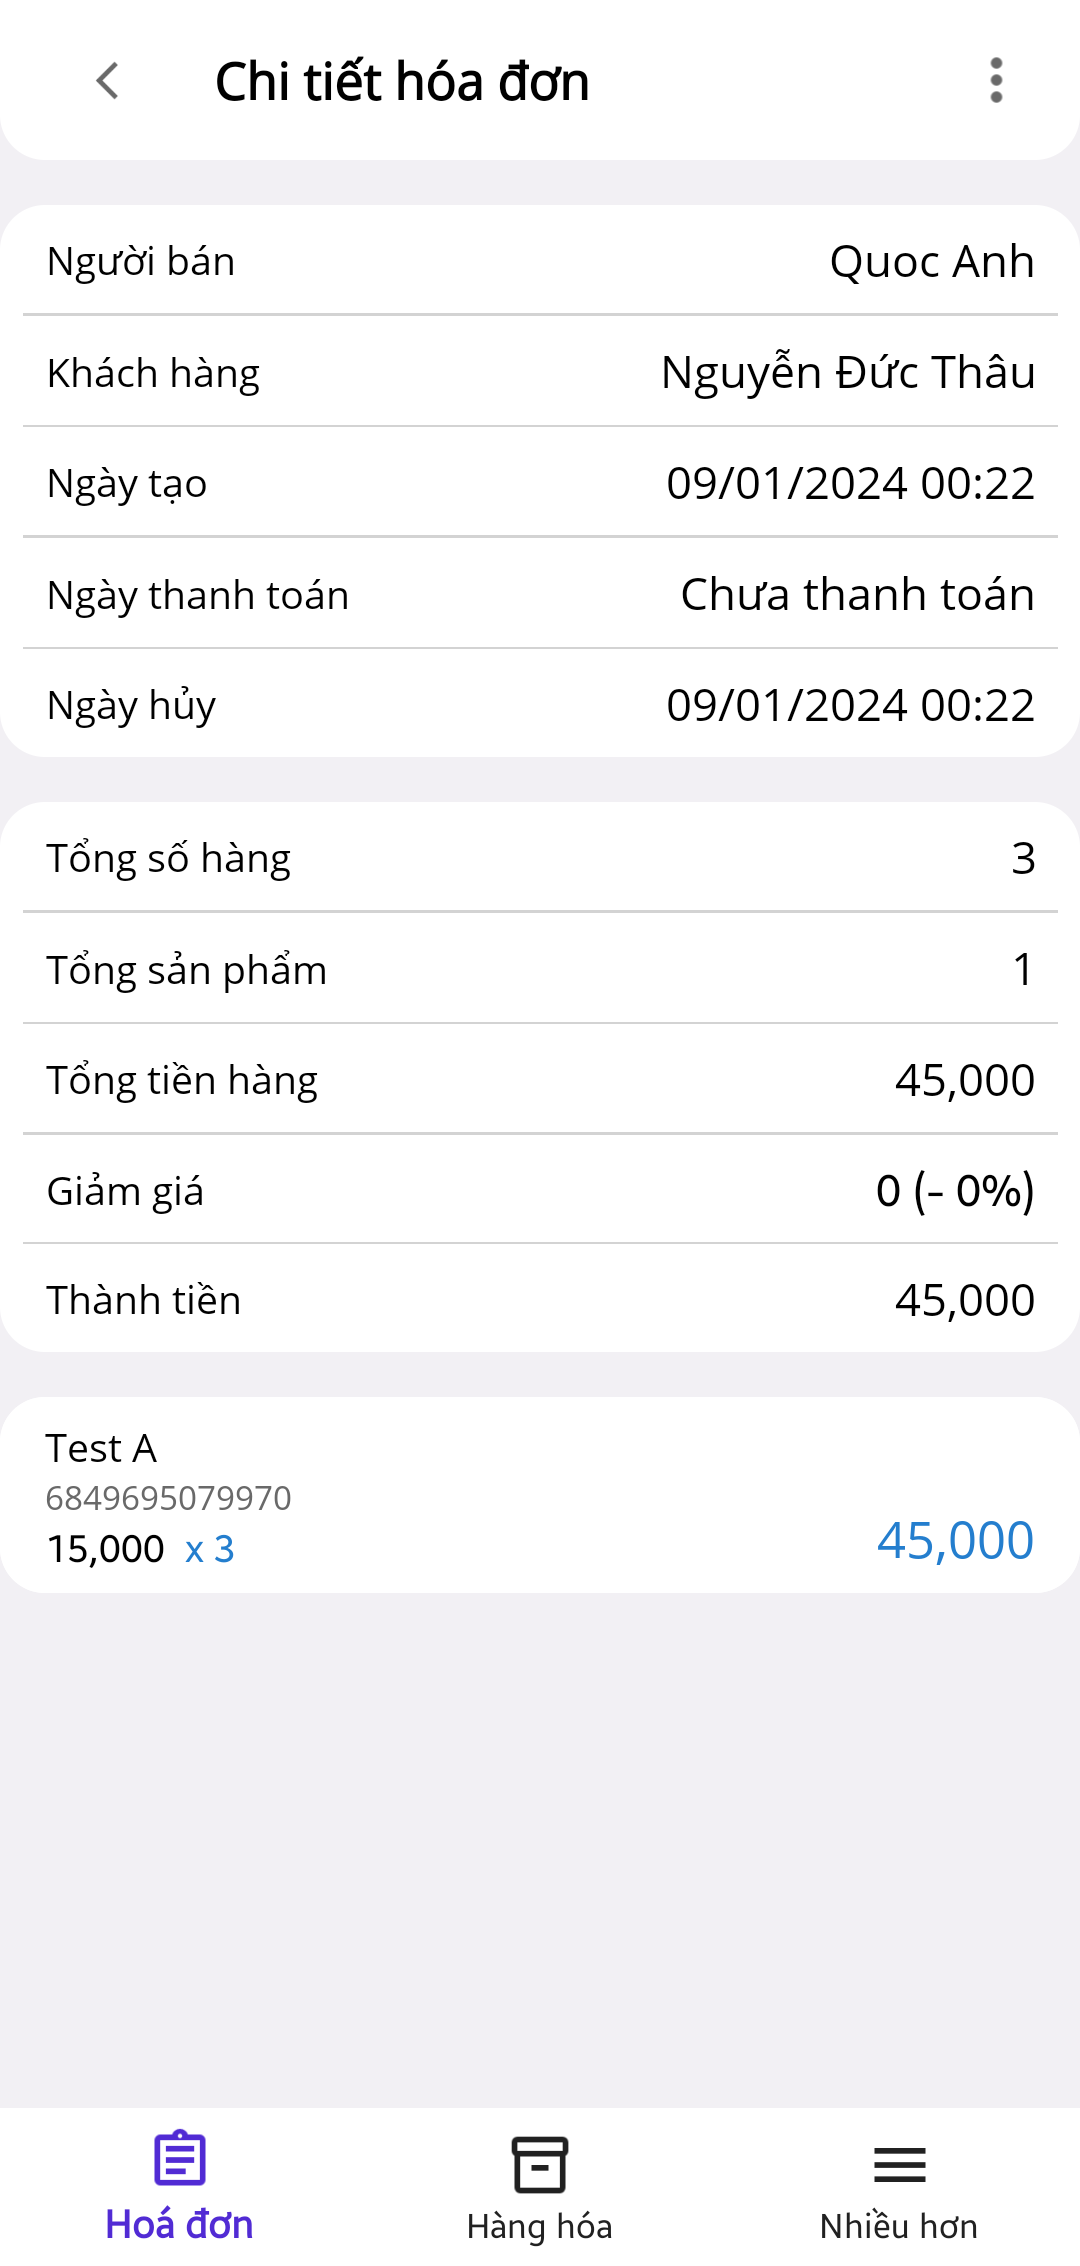
\includegraphics[width=0.9\linewidth]{Hinhve/design/screens/InvoiceDetailsPage}
        \caption{Màn hình chi tiết hóa đơn}
        \label{figure:screen-invoicedetailspage}
    \end{subfigure}
    \caption{Các màn hình hóa đơn}
    \label{figure:screen-invoicepages2}
\end{figure}
\break


\subsubsection{Chức năng sản phẩm}
Hình \ref{figure:screen-productlistpage} là màn hình danh sách sản phẩm. Tại đây người dùng có thể xem danh sách sản phẩm, và có thể tạo sản phẩm mới bằng cách nhấn vào nút " + " ở góc phải màn hình.

Hình \ref{figure:screen-productsearchpage} là màn hình tìm kiếm sản phẩm. Màn hình này được tạo ra hỗ trợ các chức năng khác của hệ thống, như đang trong quá trình người dùng tạo hóa đơn, tạo phiếu nhập kho, tạo phiếu xuất kho, v.v. Người dùng có thể tìm kiếm bằng tên hay quét mã vạch sản phẩm.
\begin{figure}[H]
    \begin{subfigure}{0.49\linewidth}
        \centering
        \includegraphics[width=0.9\linewidth]{Hinhve/design/screens/ProductListPage}
        \caption{Màn hình danh sách sản phẩm}
        \label{figure:screen-productlistpage}
    \end{subfigure}
    \begin{subfigure}{0.5\linewidth}
        \centering
        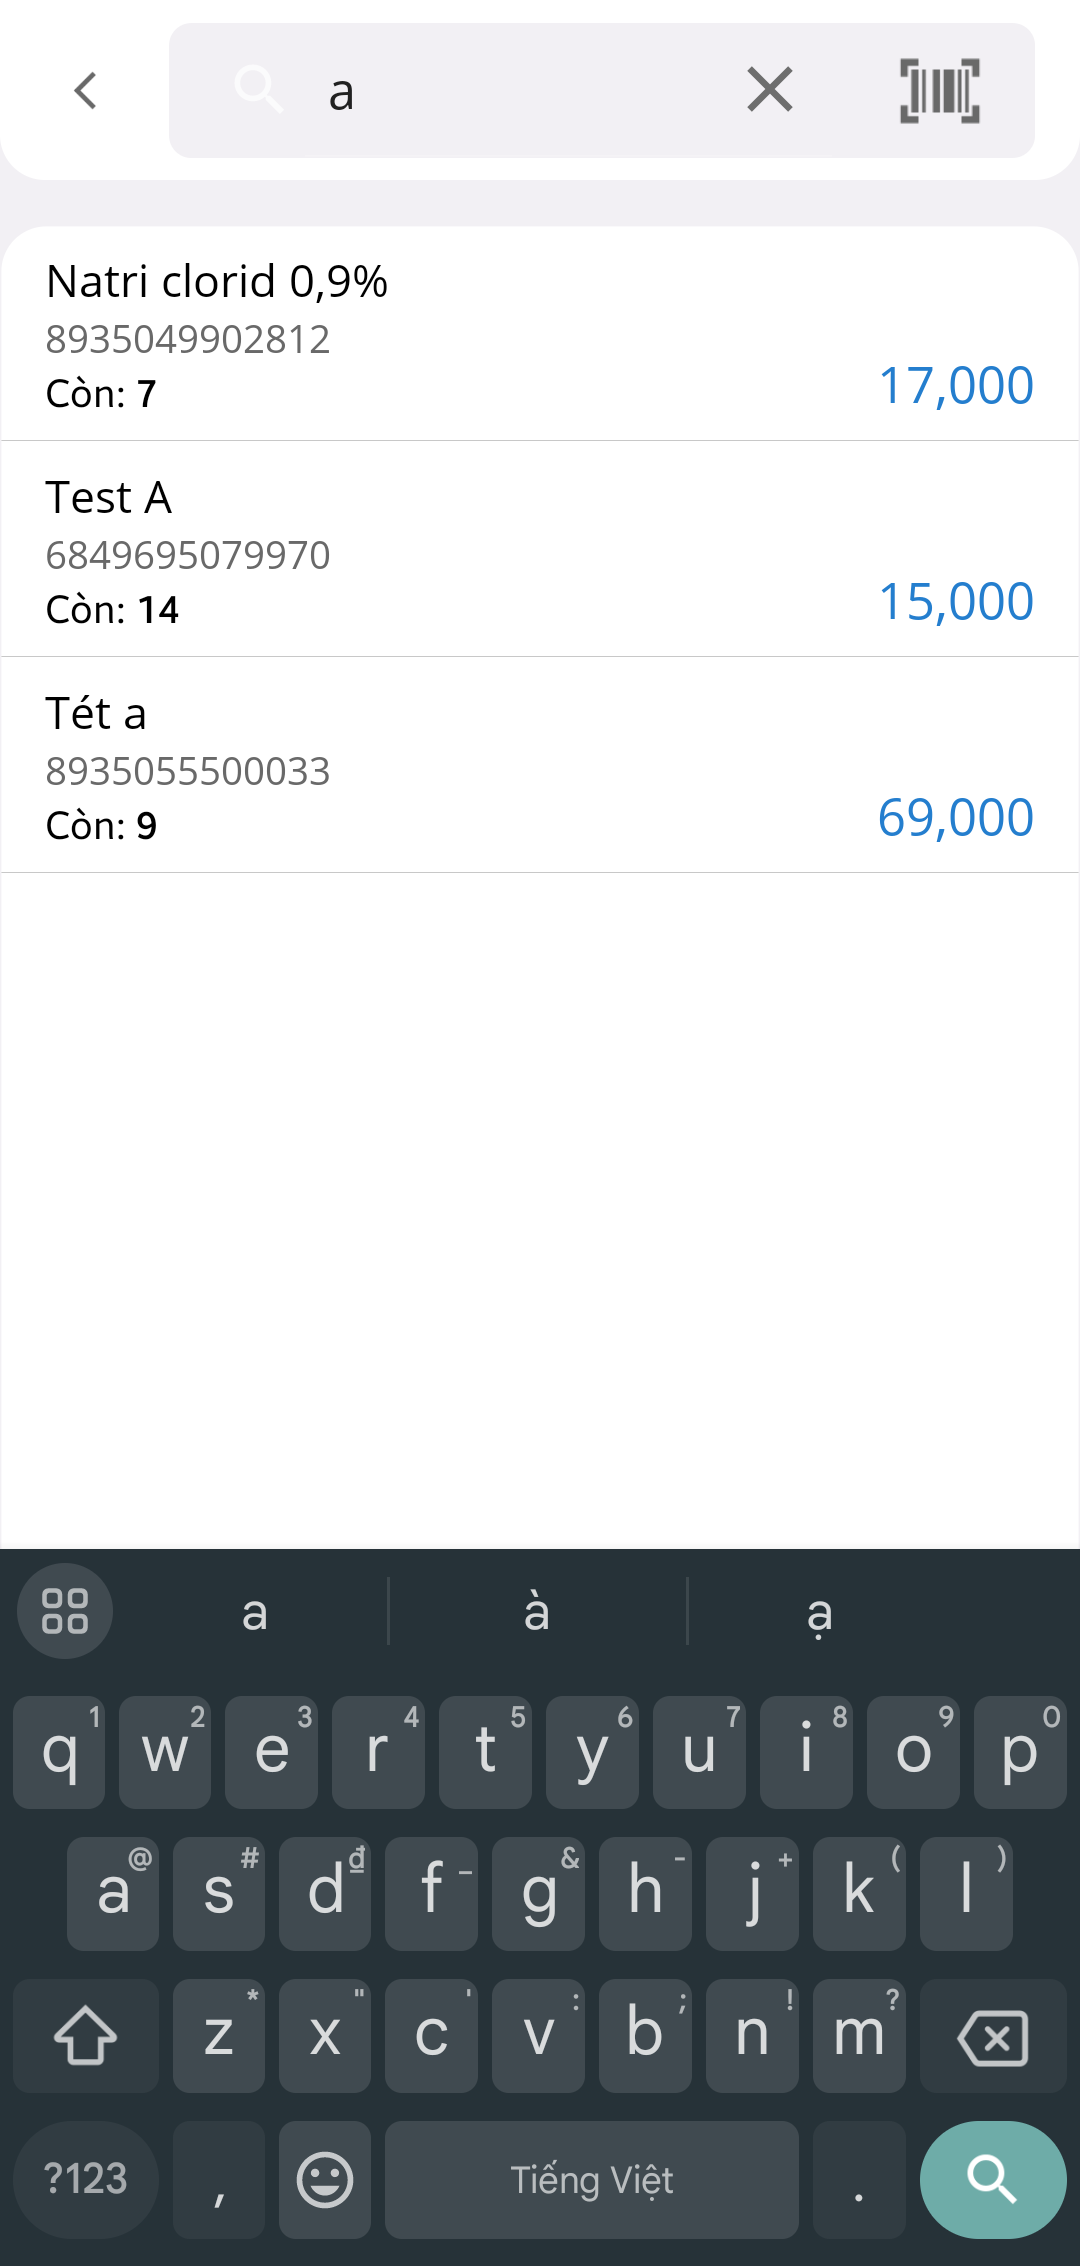
\includegraphics[width=0.9\linewidth]{Hinhve/design/screens/ProductSearchPage}
        \caption{Màn hình tìm kiếm sản phẩm}
        \label{figure:screen-productsearchpage}
    \end{subfigure}
    \caption{Các màn hình sản phẩm}
    \label{figure:screen-productpages1}
\end{figure}
\break

Hình \ref{figure:screen-productdetailspage} là màn hình chi tiết sản phẩm. Tại đây người dùng có thể xem chi tiết sản phẩm, và có thể cập nhật hay xóa sản phẩm bằng cách nhấn vào nút " \vdots{} " ở góc phải màn hình.

Hình \ref{figure:screen-productupdatepage} là màn hình cập nhật sản phẩm. Màn hình này có cấu trúc tương tự như màn hình tạo mới sản phẩm, nhưng có thêm một số trường thông tin đã được điền sẵn khi người dùng chọn sửa sản phẩm từ màn hình chi tiết.
\begin{figure}[H]
    \begin{subfigure}{0.49\linewidth}
        \centering
        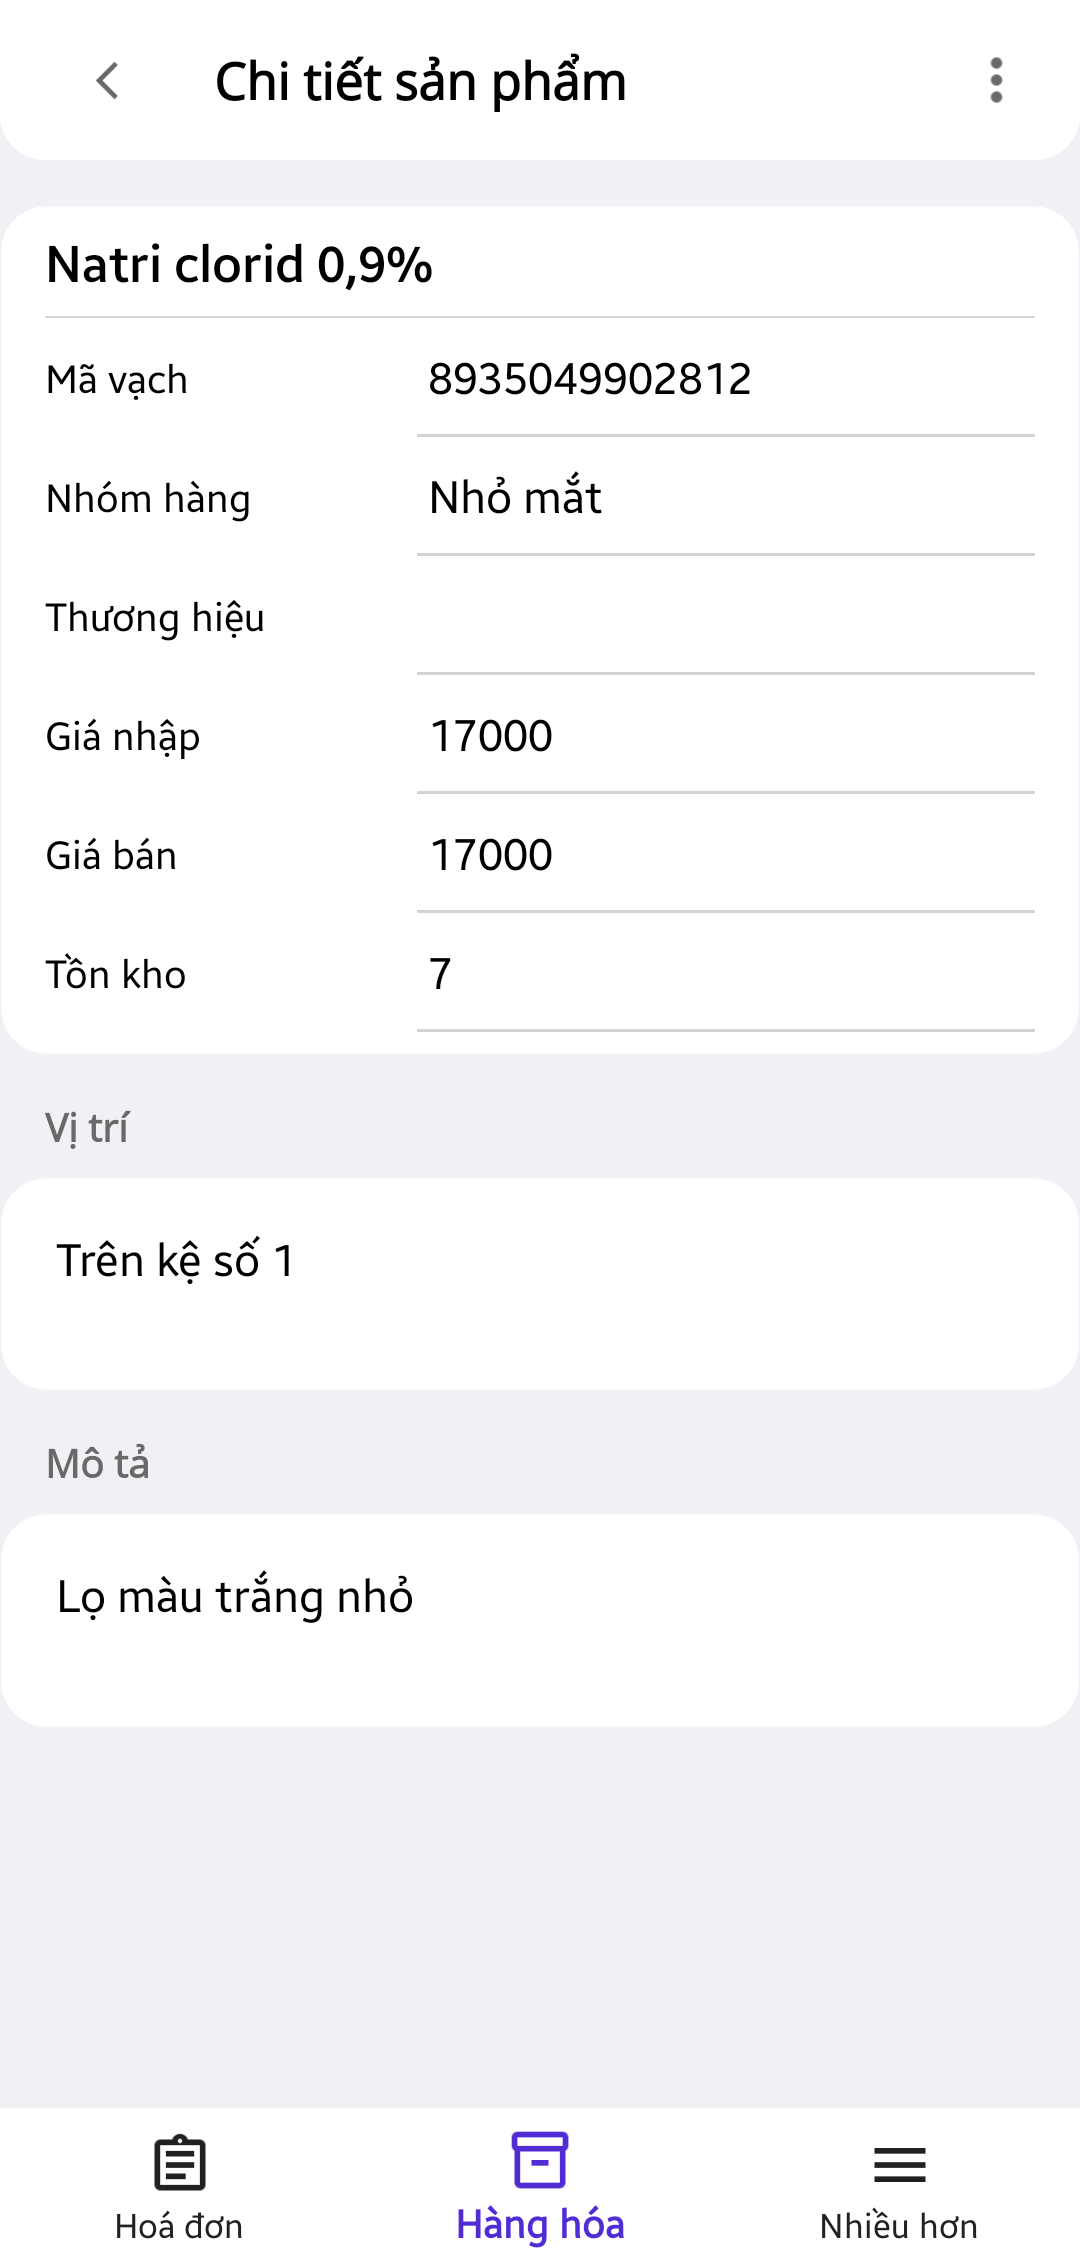
\includegraphics[width=0.9\linewidth]{Hinhve/design/screens/ProductDetailsPage}
        \caption{Màn hình chi tiết sản phẩm}
        \label{figure:screen-productdetailspage}
    \end{subfigure}
    \begin{subfigure}{0.5\linewidth}
        \centering
        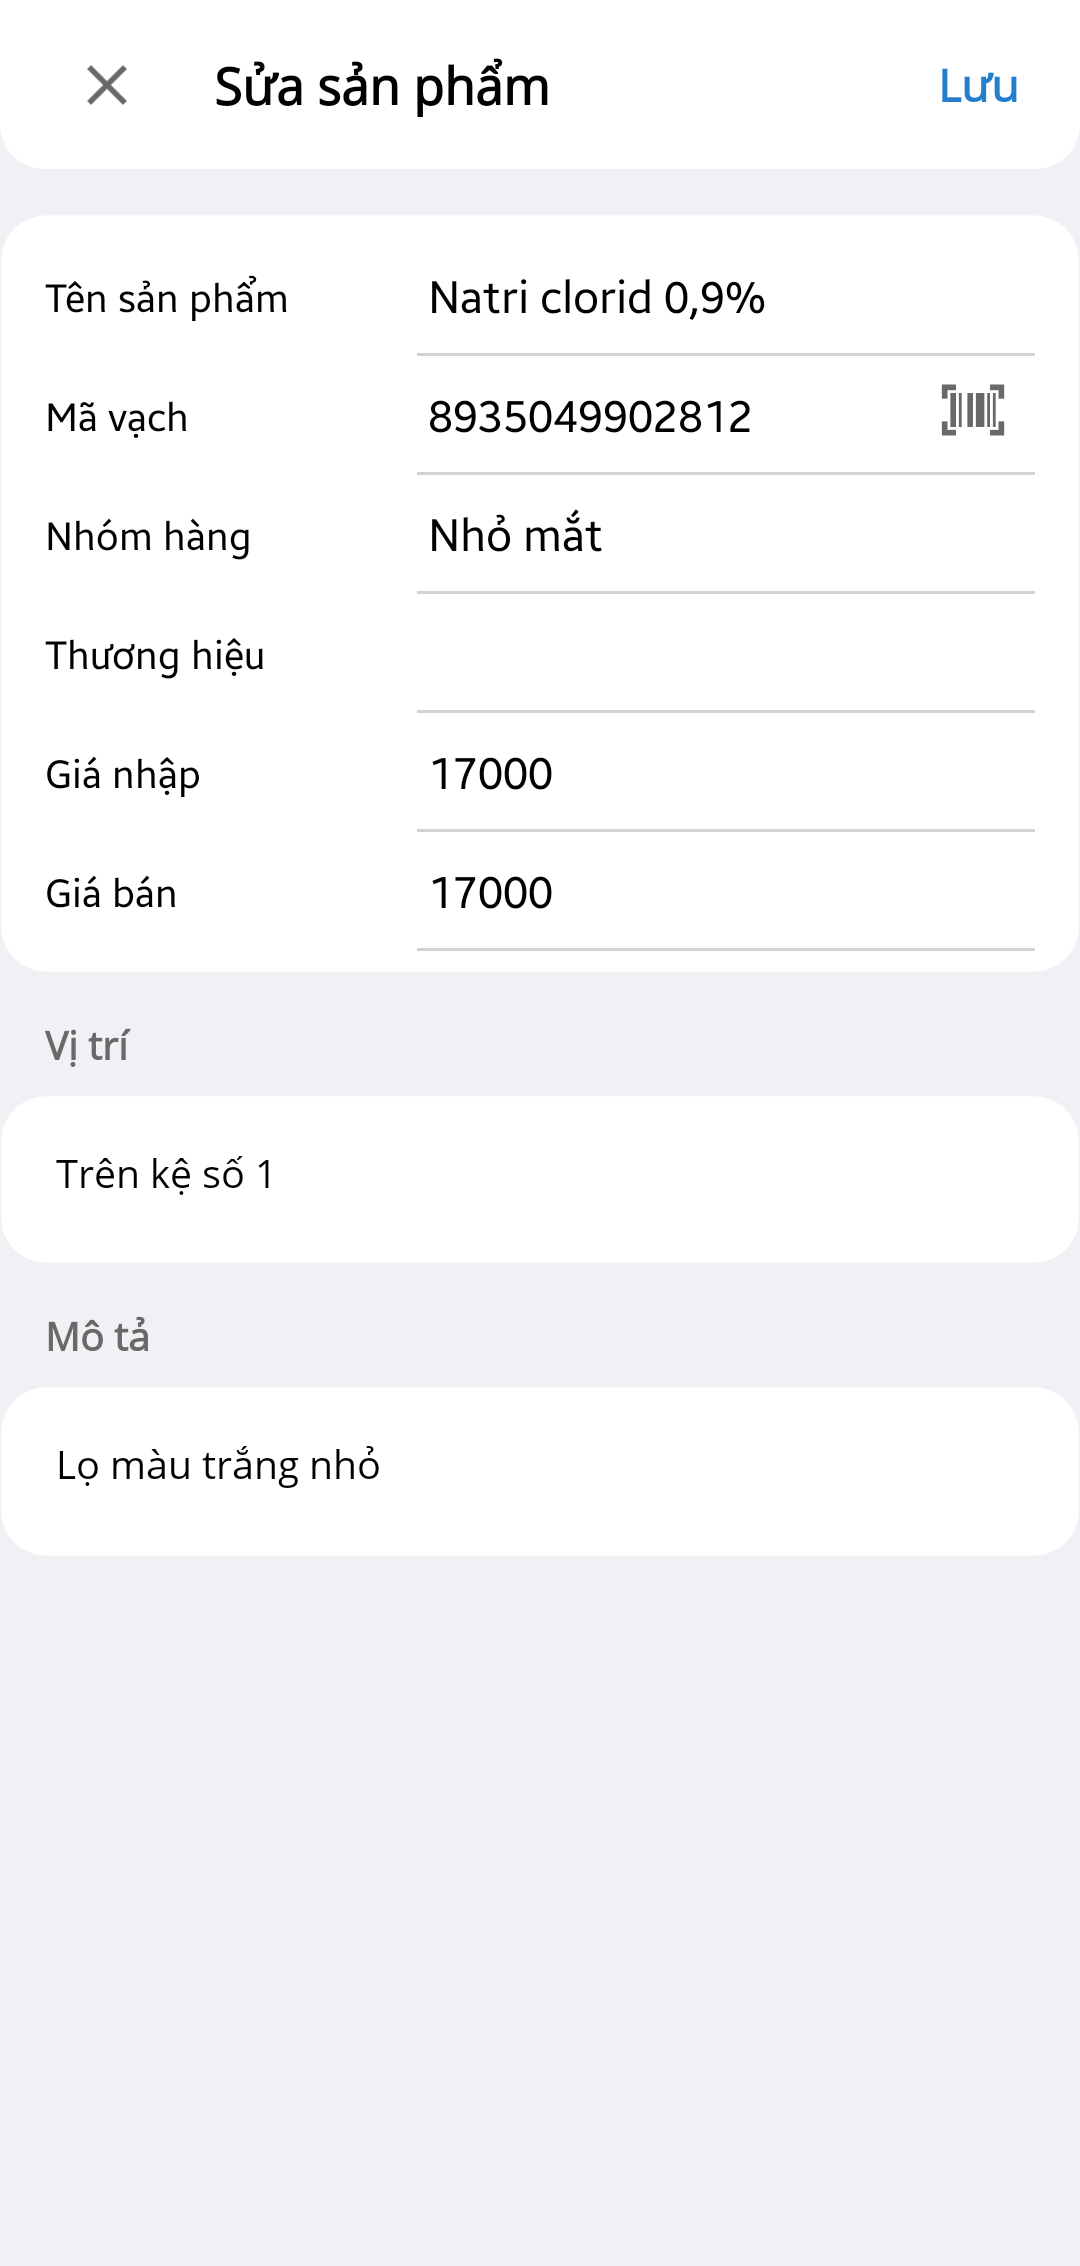
\includegraphics[width=0.9\linewidth]{Hinhve/design/screens/ProductUpdatePage}
        \caption{Màn hình cập nhật sản phẩm}
        \label{figure:screen-productupdatepage}
    \end{subfigure}
    \caption{Các màn hình sản phẩm}
    \label{figure:screen-productpages2}
\end{figure}
\break

\subsubsection{Các chức năng khác}
Do hệ thống có cấu trúc giao diện gần tương tự nhau rất nhiều, sau đây là các màn hình của một phần các chức năng khác để minh họa nhanh.

Hình \ref{figure:screen-clientlistpage} là màn hình danh sách khách hàng. Người dùng có thể tạo khách hàng mới bằng cách nhấn vào nút " + " ở góc phải màn hình.

Hình \ref{figure:screen-exportreportcreatepage} là màn hình tạo phiếu xuất kho. Tại đây người dùng có thể thêm sản phẩm vào phiếu xuất kho bằng cách nhấn vào nút " + Thêm ". Ngoài ra, để xóa sản phẩm khỏi phiếu xuất kho, người dùng có thể vuốt sang trái sản phẩm hay vuốt sang phải để xem chi tiết hơn sản phẩm đó.
\begin{figure}[H]
    \begin{subfigure}{0.49\linewidth}
        \centering
        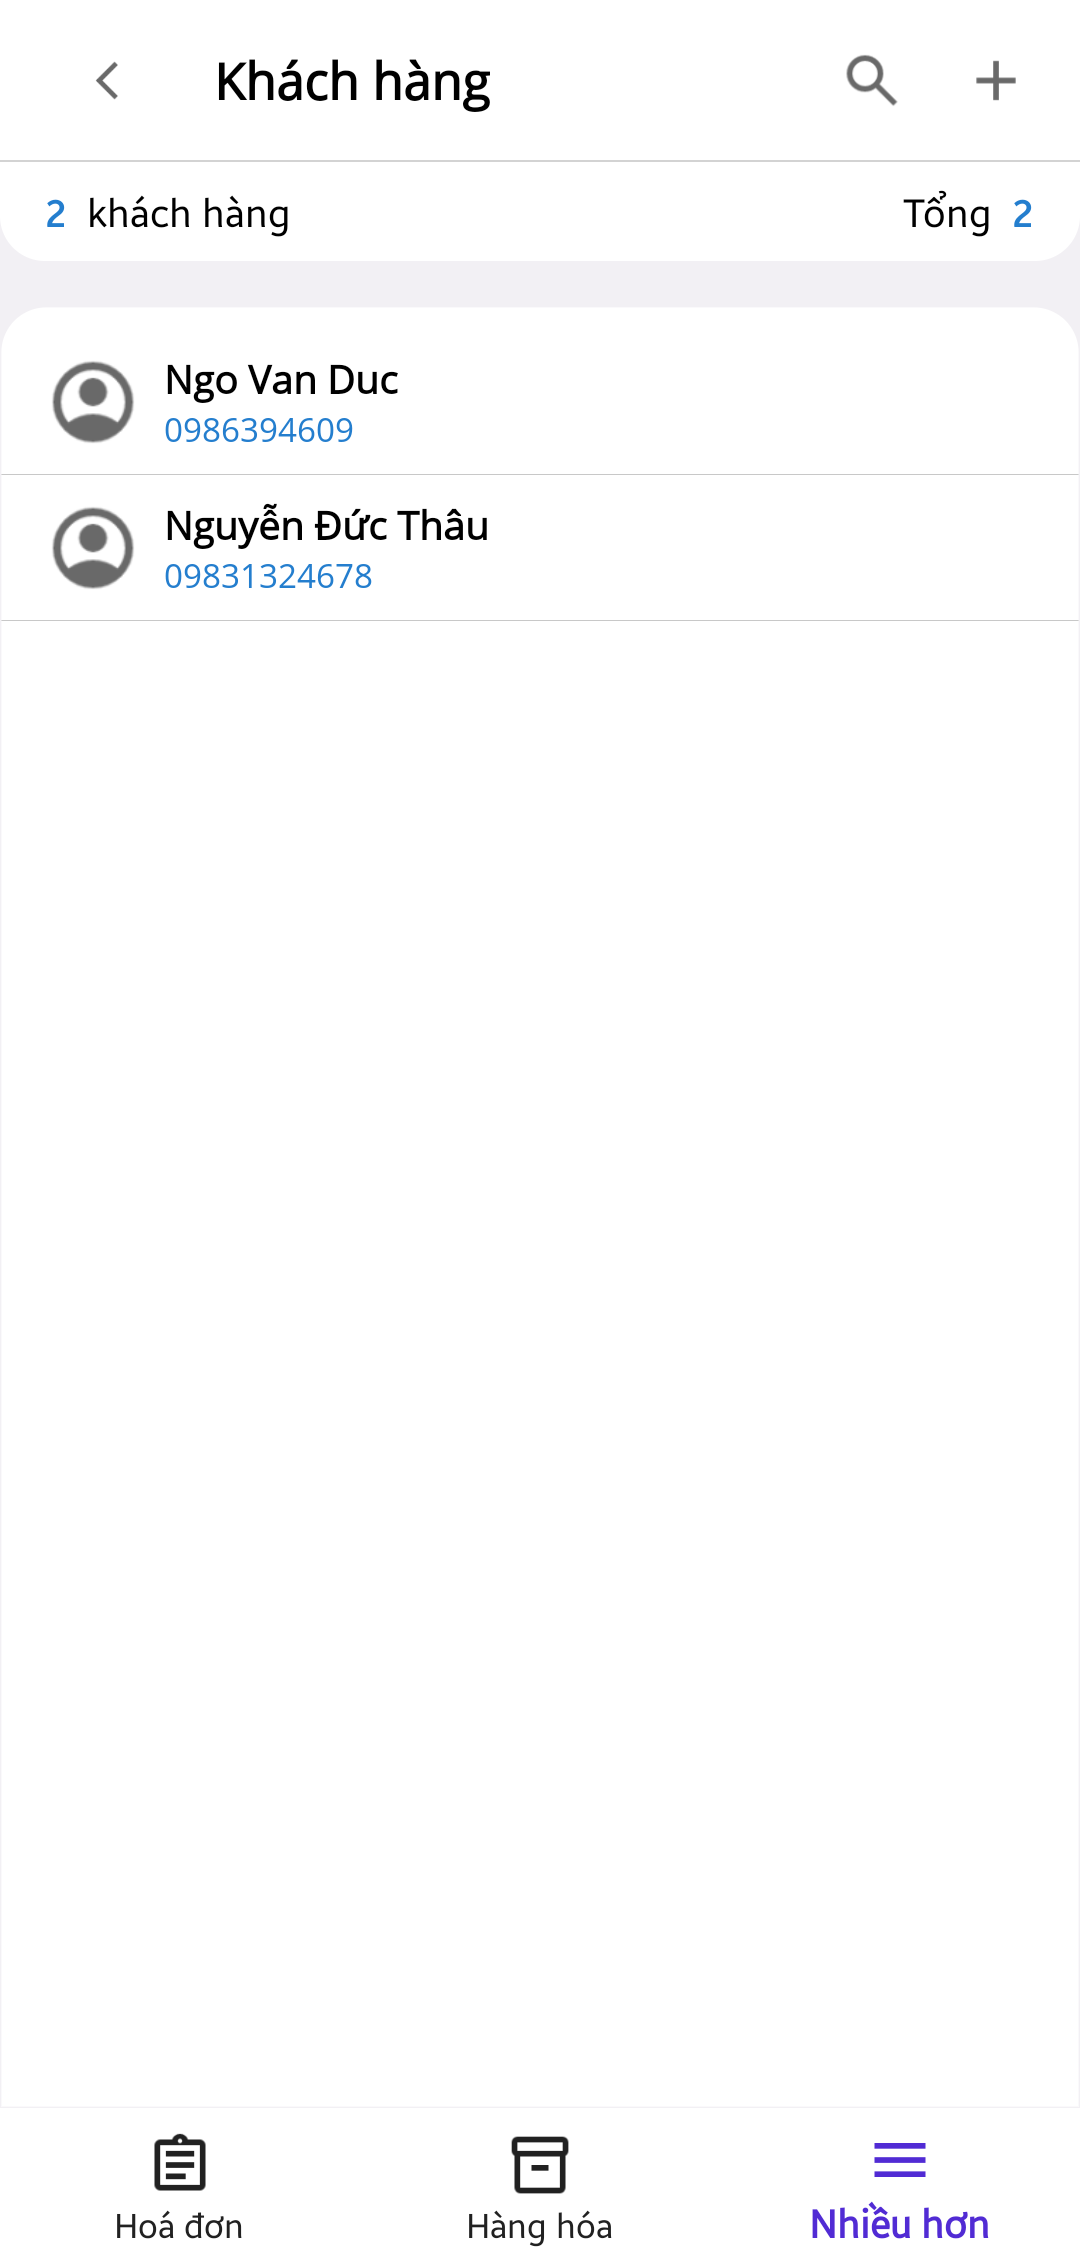
\includegraphics[width=0.9\linewidth]{Hinhve/design/screens/ClientListPage}
        \caption{Màn hình danh sách khách hàng}
        \label{figure:screen-clientlistpage}
    \end{subfigure}
    \begin{subfigure}{0.5\linewidth}
        \centering
        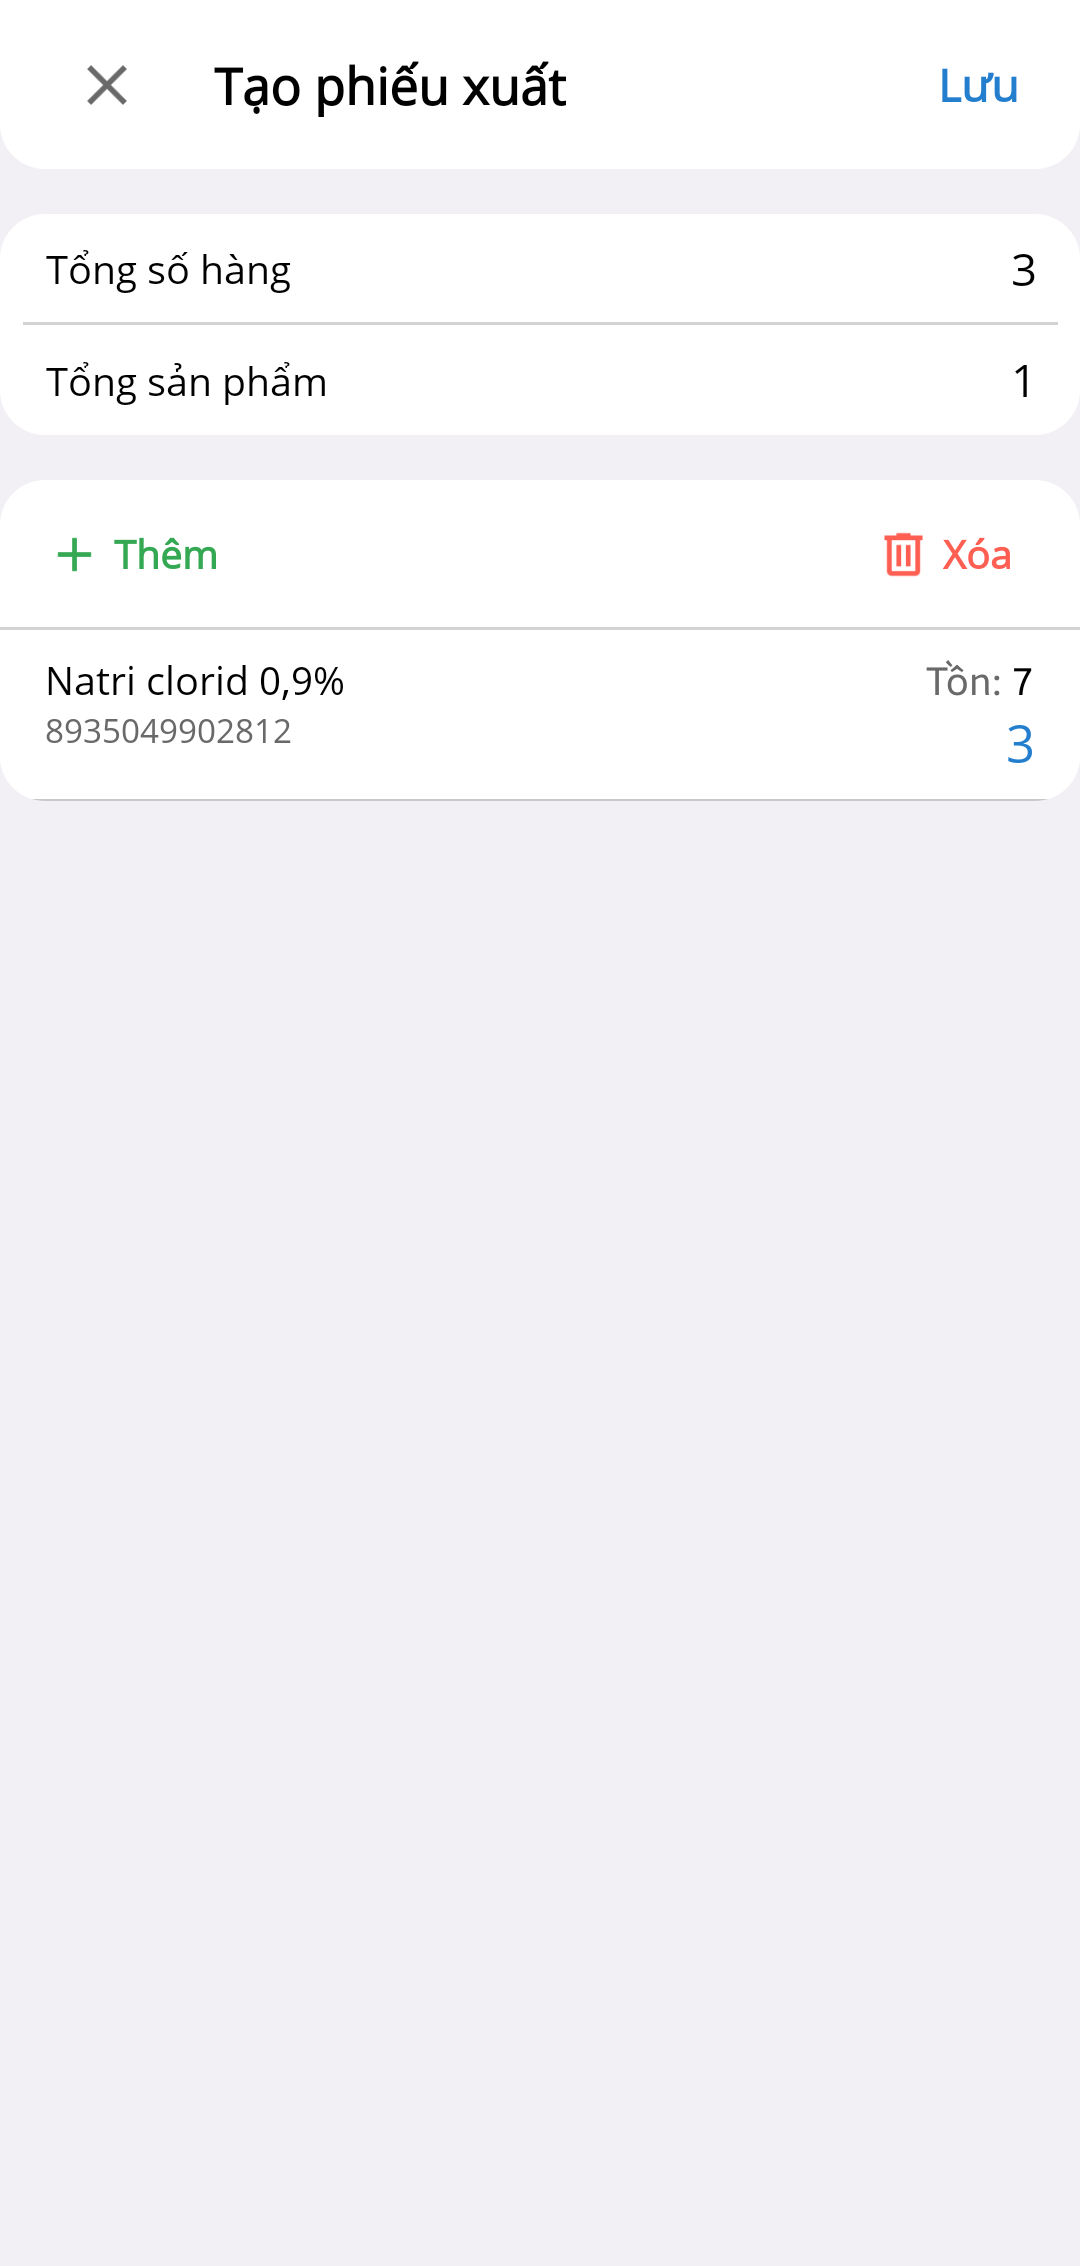
\includegraphics[width=0.9\linewidth]{Hinhve/design/screens/ExportReportCreatePage}
        \caption{Màn hình tạo phiếu xuất kho}
        \label{figure:screen-exportreportcreatepage}
    \end{subfigure}
    \caption{Các màn hình khác}
    \label{figure:screen-variouspages1}
\end{figure}
\break

Hình \ref{figure:screen-auditreportdetailspage} là màn hình chi tiết phiếu kiểm kho. Xóa phiếu kiểm kho bằng cách nhấn vào nút " \vdots{} " ở góc phải màn hình. Người dùng có thể xem chi tiết sản phẩm kiểm kho bằng cách nhấn vào sản phẩm đó mà không phải thủ công tìm sản phẩm đó.

Hình \ref{figure:screen-auditreportcreatepage} là màn hình tạo phiếu kiểm kho. Tại đây người dùng có thể thêm sản phẩm vào phiếu kiểm kho bằng cách nhấn vào nút " + Thêm ". Ngoài ra, để xóa sản phẩm khỏi phiếu kiểm kho, người dùng có thể vuốt sang trái sản phẩm hay vuốt sang phải để xem chi tiết hơn sản phẩm đó. Bấm vào sản phẩm nào đó để hiện hộp thoại chỉnh các số liệu của sản phẩm đó.
\begin{figure}[H]
    \begin{subfigure}{0.49\linewidth}
        \centering
        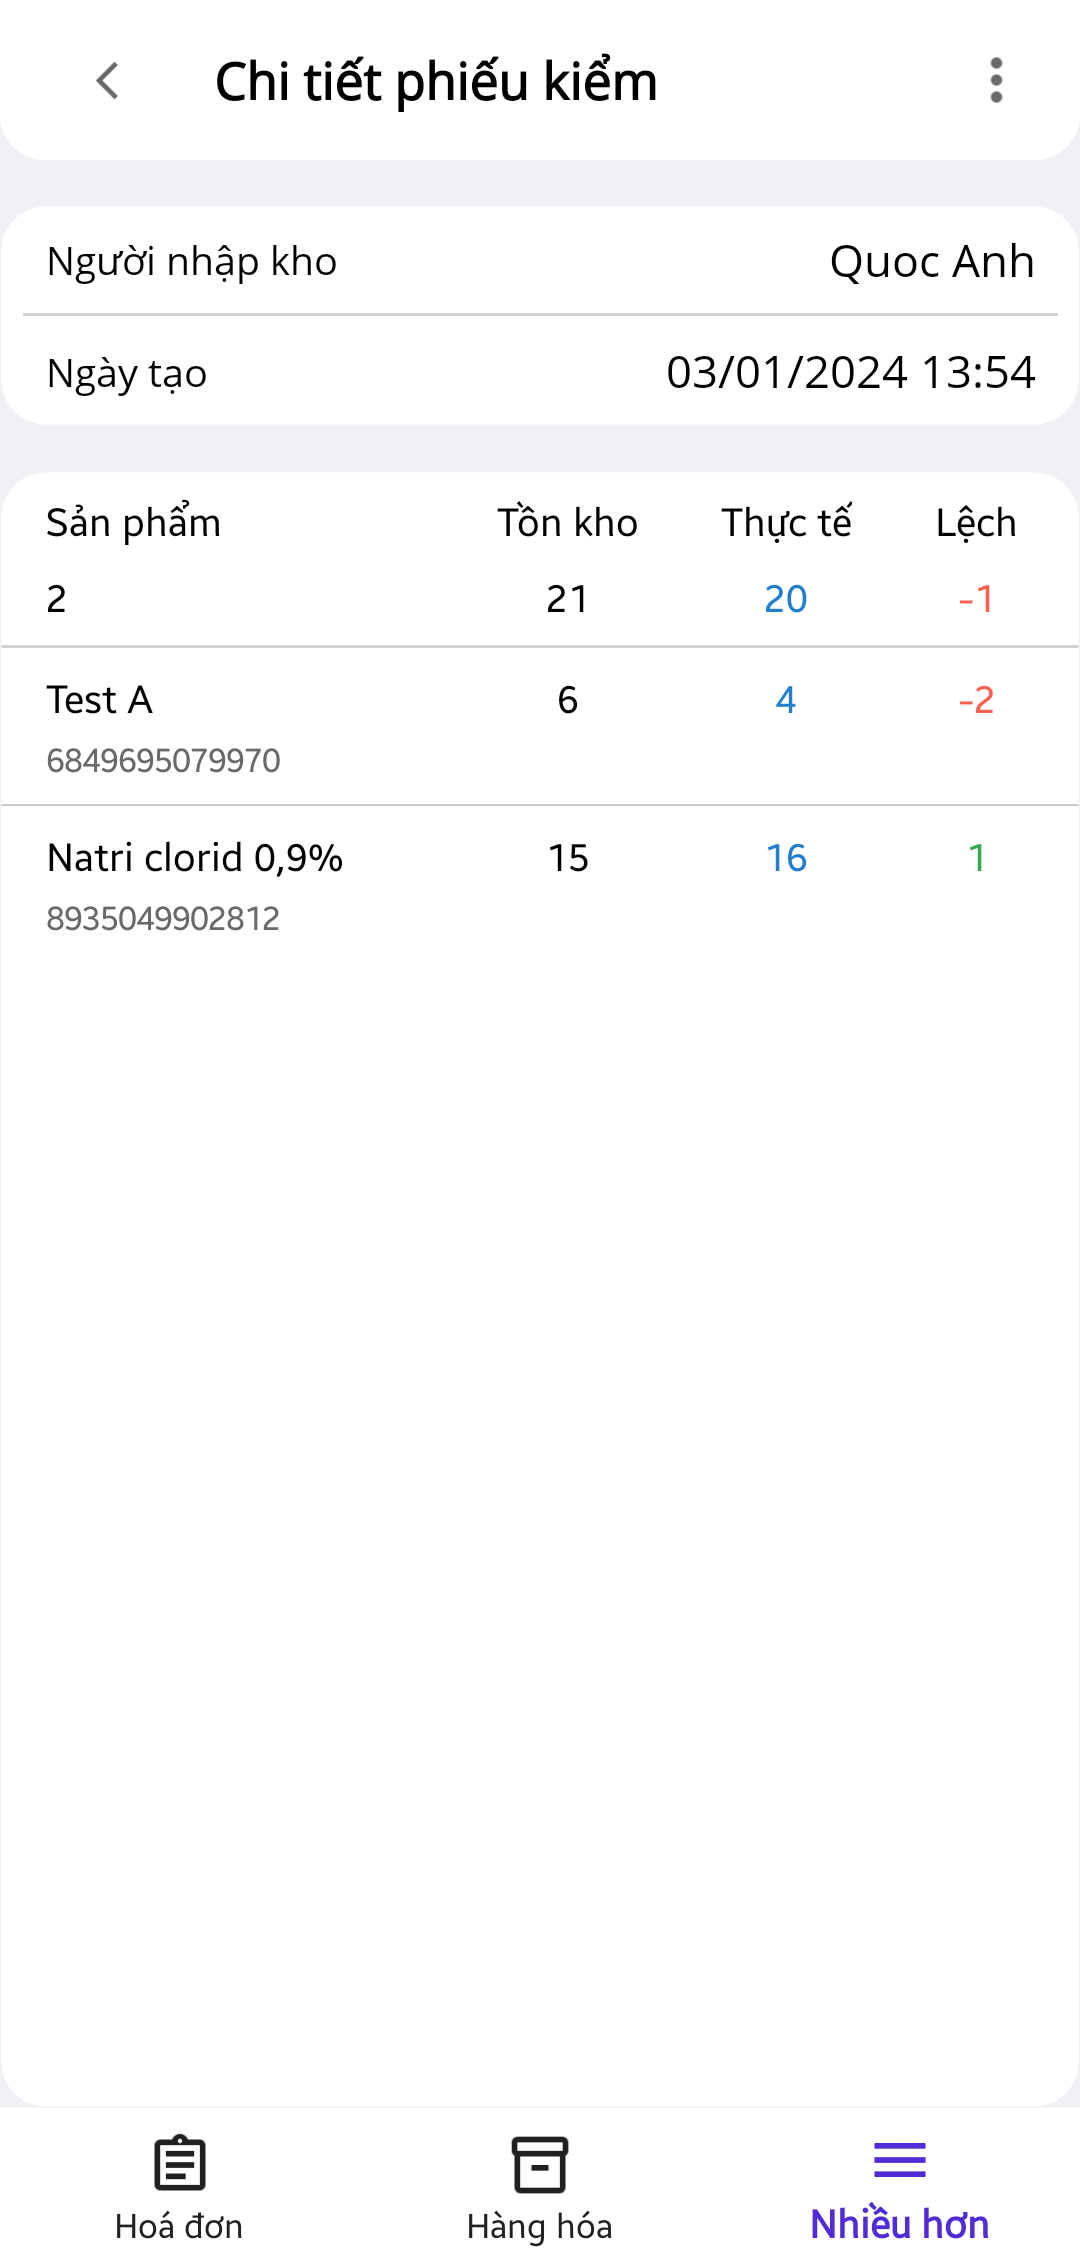
\includegraphics[width=0.9\linewidth]{Hinhve/design/screens/AuditReportDetailsPage}
        \caption{Màn hình chi tiết phiếu kiểm kho}
        \label{figure:screen-auditreportdetailspage}
    \end{subfigure}
    \begin{subfigure}{0.5\linewidth}
        \centering
        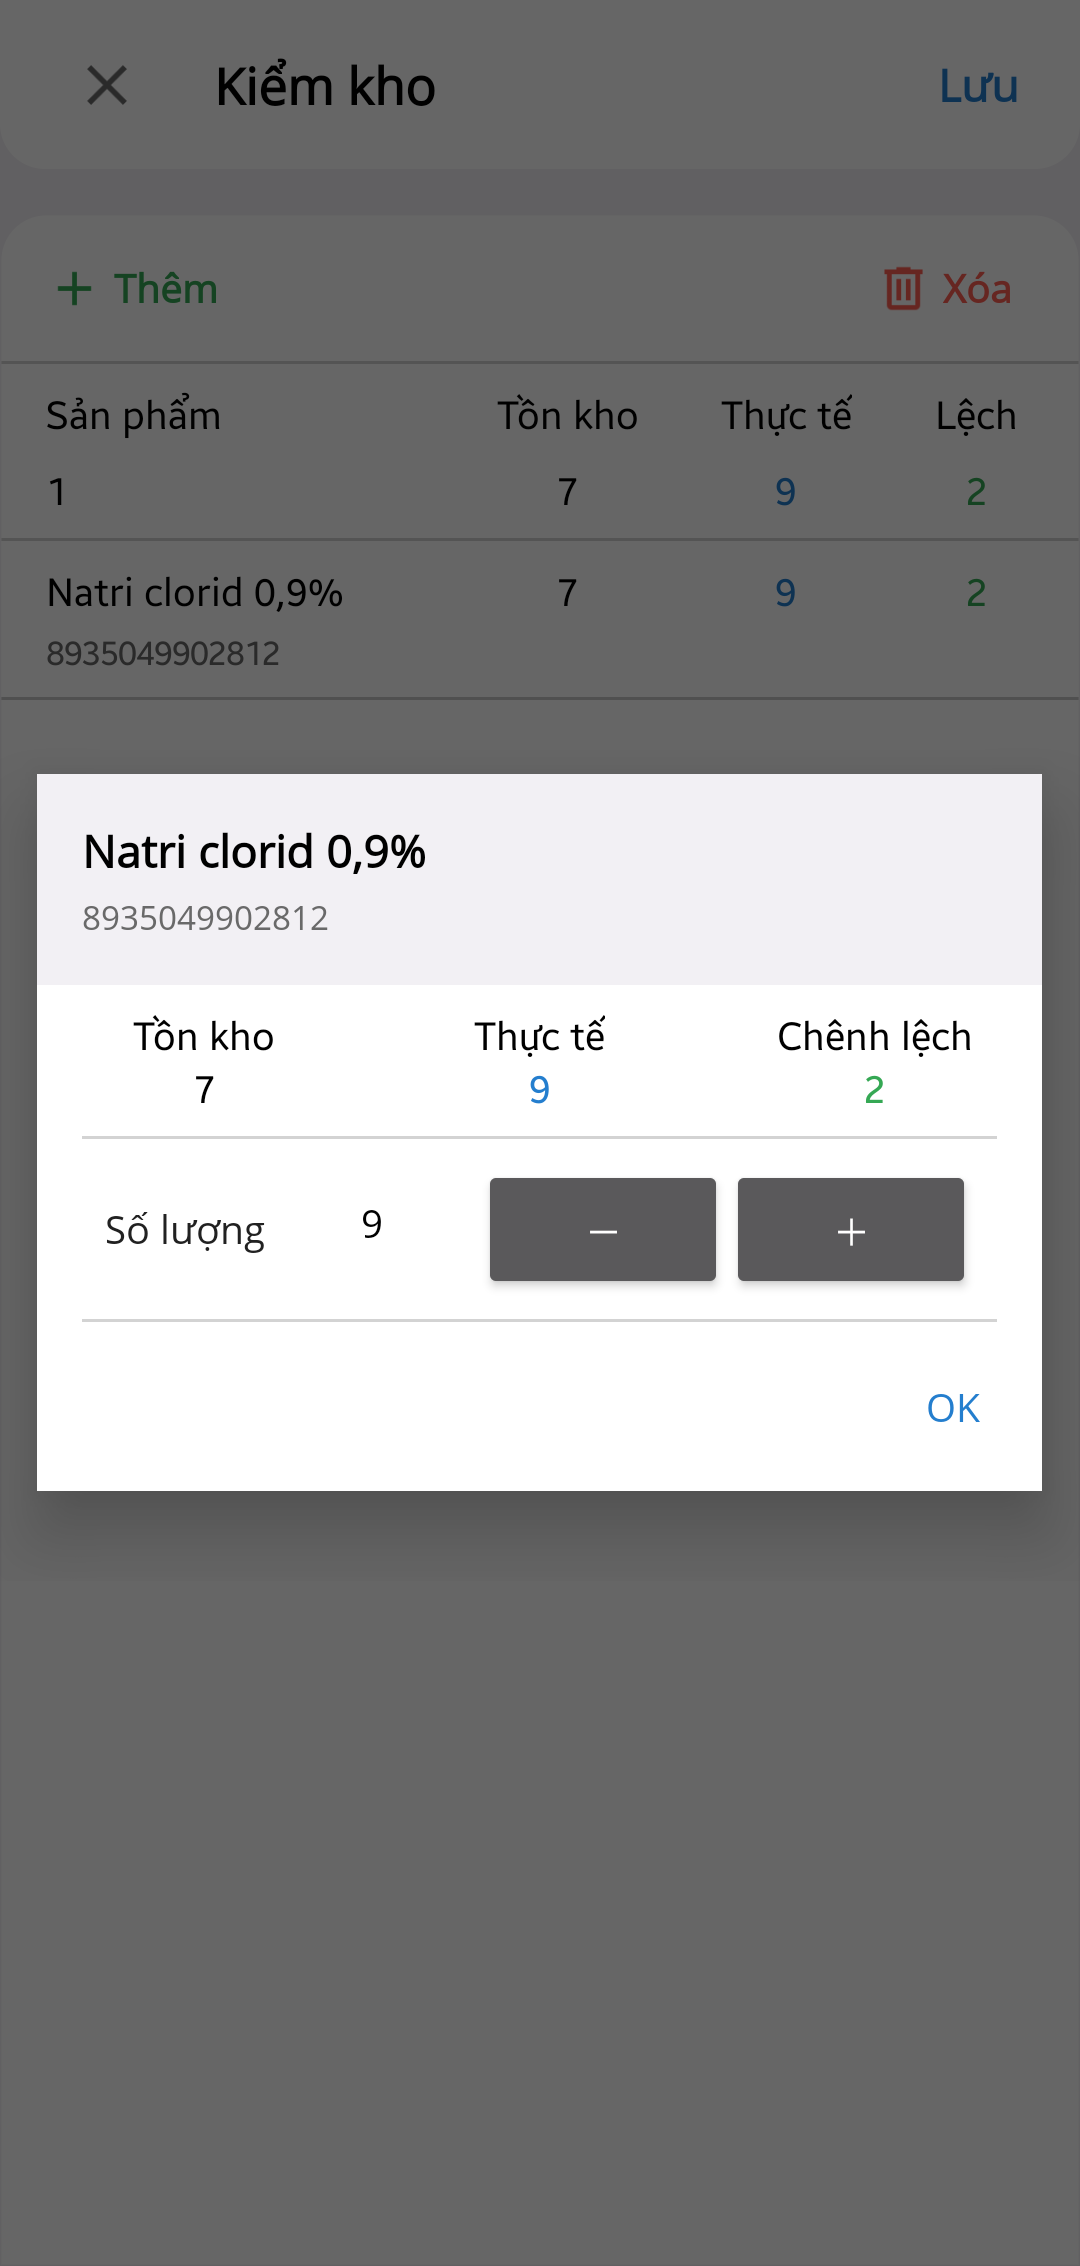
\includegraphics[width=0.9\linewidth]{Hinhve/design/screens/AuditReportCreatePage}
        \caption{Màn hình tạo phiếu kiểm kho}
        \label{figure:screen-auditreportcreatepage}
    \end{subfigure}
    \caption{Các màn hình khác}
    \label{figure:screen-variouspages2}
\end{figure}
\break


\section{Kiểm thử}
% Phần này có độ dài từ hai đến ba trang. Sinh viên thiết kế các trường hợp kiểm thử cho hai đến ba chức năng quan trọng nhất. Sinh viên cần chỉ rõ các kỹ thuật kiểm thử đã sử dụng. Chi tiết các trường hợp kiểm thử khác, nếu muốn trình bày, sinh viên đưa vào phần phụ lục.
% Sinh viên sau cùng tổng kết về số lượng các trường hợp kiểm thử và kết quả kiểm thử. Sinh viên cần phân tích lý do nếu kết quả kiểm thử không đạt.
Các chức năng kiểm thử chính được lựa chọn ở đây là để một phần phản ánh lại khả năng của hệ thống, các kịch bản kiểm thử khác quá dài và không thể trình bày hết trong báo cáo này. Các kịch bản được mô tả trong bảng \ref{table:testcases}.
\begin{xltabular}{\textwidth}{|l|>{\raggedright\arraybackslash}p{2cm}|>{\raggedright\arraybackslash}X|>{\raggedright\arraybackslash}X|c|}
    \caption{Các kịch bản kiểm thử} \label{table:testcases} \\
    \hline
    \multicolumn{1}{|c|}{\textbf{Mã}} & \multicolumn{1}{c|}{\textbf{Mô tả}}                     & \multicolumn{1}{c|}{\textbf{Quy trình}}                                                                         & \multicolumn{1}{c|}{\textbf{Kết quả mong đợi}}                                                                                                                                                   & \multicolumn{1}{c|}{\textbf{Đạt?}} \\ \hline
    \endfirsthead

    \hline
    \multicolumn{5}{|c|}{Tiếp của bảng \ref{table:testcases}} \\ \hline
    \multicolumn{1}{|c|}{\textbf{Mã}} & \multicolumn{1}{c|}{\textbf{Mô tả}}                     & \multicolumn{1}{c|}{\textbf{Quy trình}}                                                                         & \multicolumn{1}{c|}{\textbf{Kết quả mong đợi}}                                                                                                                                                   & \multicolumn{1}{c|}{\textbf{Đạt?}} \\ \hline
    \endhead

    TC01 & Đăng nhập                                           & 1. Nhập tên đăng nhập, mật khẩu đúng                                                                        & Tự động chuyển sang màn hình chính                                                                                                                                                           & Đạt \\ \hline
    TC02 & Đăng nhập                                           & 1. Nhập tên đăng nhập, mật khẩu sai                                                                         & Hiện thông báo lỗi                                                                                                                                                                           & Đạt \\ \hline
    TC03 & Tìm hóa đơn bằng tên sản phẩm                       & 1. Nhập từ khóa "Natri" \newline 2. Chọn nút "Tìm kiếm"                                                     & Chuyển sang màn hình danh sách và hiện hóa đơn có sản phẩm tên chứa "Natri"                                                                                                                  & Đạt \\ \hline
    TC04 & Tìm hóa đơn bằng mã vạch sản phẩm                   & 1. Bấm nút hình mã vạch \newline 2. Quay camera về mã vạch sản phẩm "8642314687523"                         & Chuyển sang màn hình danh sách và hiện hóa đơn có sản phẩm mã vạch "8642314687523"                                                                                                           & Đạt \\ \hline
    TC05 & Bỏ trống tất cả các trường tìm kiếm hóa đơn         & 1. Bỏ trống tất cả các trường \newline 2. Chọn nút "Tìm kiếm"                                               & Hiện tất cả hóa đơn                                                                                                                                                                          & Đạt \\ \hline
    TC06 & Thêm sản phẩm hết hàng vào phiếu tạo hóa đơn        & 1. Chọn nút "+ Thêm" \newline 2. Nhập tên sản phẩm "Natri" và bấm tìm \newline 3. Chọn sản phẩm có "Còn: 0" & 1. Hiện màn hình tìm kiếm sản phẩm \newline 2. Hiện danh sách sản phẩm chứa tên "Natri" \newline 3. Quay về màn hình tạo hóa đơn và hiện thông báo lỗi "Hết hàng"                            & Đạt \\ \hline
    TC07 & Thêm sản phẩm vào phiếu tạo hóa đơn                 & 1. Chọn nút "+ Thêm" \newline 2. Nhập tên sản phẩm "Trà" và bấm tìm \newline 3. Chọn "Trà Actiso"           & 1. Hiện màn hình tìm kiếm sản phẩm \newline 2. Hiện danh sách sản phẩm chứa tên "Trà" \newline 3. Quay về màn hình tạo hóa đơn và hiện sản phẩm đã chọn trong danh sách sản phẩm của hóa đơn & Đạt \\ \hline
    TC08 & Chỉnh số lượng sản phẩm bán trong phiếu tạo hóa đơn & 1. Chọn sản phẩm "Trà Actiso" \newline 2. Bấm dấu cộng 3 lần \newline 3. Chọn "OK"                          & 1. Hiện hộp thoại chỉnh số lượng \newline 2. Số lượng tăng lên "4" \newline 3. Quay về màn hình tạo hóa đơn, sản phẩm hiện "20,000 x 4" "80,000" và thanh "Thành tiền" tăng lên 80000        & Đạt \\ \hline
    TC09 & Hoàn thành tạo hóa đơn đã thanh toán                & 1. Tích ô "Đã thanh toán" \newline 2. Chọn nút "Lưu"                                                        & Quay về màn hình danh sách hóa đơn và hiển thị lại trang có hóa đơn đã thanh toán mới nhất                                                                                                   & Đạt \\ \hline
    TC10 & Tạo thêm sản phẩm mới                               & 1. Chọn nút "+" \newline 2. Nhập các trường và chọn nút "Lưu"                                               & 1. Hiện màn hình tạo mới sản phẩm \newline 2. Quay về màn hình danh sách sản phẩm và hiện sản phẩm đã thêm trong danh sách sản phẩm                                                          & Đạt \\ \hline
    TC11 & Xóa sản phẩm                                        & 1. Chọn sản phẩm trong màn hình danh sách sản phẩm \newline 2. Chọn nút " \vdots{} " $\rightarrow$ "Xóa"    & 1. Hiện màn hình chi tiết sản phẩm \newline 2. Quay về màn hình danh sách sản phẩm và sản phẩm không còn trong danh sách sản phẩm                                                            & Đạt \\ \hline
    TC12 & Cập nhật sản phẩm                                   & 1. Chọn sản phẩm trong màn hình danh sách sản phẩm \newline 2. Chọn nút " \vdots{} " $\rightarrow$ "Sửa"    & 1. Hiện màn hình chi tiết sản phẩm \newline 2. Hiện màn hình sửa sản phẩm với các trường đã được điền sẵn \newline 3. Quay về màn hình chi tiết sản phẩm với thông tin mới                   & Đạt \\ \hline
    TC13 & Làm mới màn hình danh sách sản phẩm                 & 1. Kéo từ giữa màn hình xuống dưới một đoạn cho hiện vòng tròn                                              & Màn hình danh sách làm mới dữ liệu và vòng tròn biến mất                                                                                                                                     & Đạt \\ \hline
    TC14 & Xem chi tiết sản phẩm trong phiếu nhập kho          & 1. Chọn phiếu nhập trong màn hình danh sách nhập kho \newline 2. Chọn sản phẩm                              & 1. Hiện màn hình chi tiết phiếu nhập kho \newline 2. Hiện màn hình chi tiết sản phẩm                                                                                                         & Đạt \\ \hline
    TC15 & Hủy phiếu nhập kho                                  & 1. Chọn phiếu nhập trong màn hình danh sách nhập kho \newline 2. Chọn nút " \vdots{} " $\rightarrow$ "Hủy"  & 1. Hiện màn hình chi tiết phiếu nhập kho \newline 2. Màn hình chi tiết được làm mới và hiện thêm trường "Ngày hủy phiếu" với thời gian hủy                                                   & Đạt \\ \hline
    TC16 & Xem chi tiết sản phẩm trước khi chọn                & 1. Hiện trang tìm kiếm sản phẩm và tìm kiếm \newline 2. Quẹt phải một sản phẩm để hiện chữ "Info"           & 1. Hiện màn hình tìm kiếm sản phẩm \newline 2. Hiện danh sách sản phẩm \newline 3. Hiện màn hình chi tiết sản phẩm                                                                           & Đạt \\ \hline
    TC17 & Đăng xuất                                           & 1. Chọn nút hình mũi nên chỉ cửa màu đỏ                                                                     & Quay về màn hình đăng nhập                                                                                                                                                                   & Đạt \\ \hline
\end{xltabular}


\section{Triển khai}
\label{section:deployment}
% Sinh viên trình bày mô hình và/hoặc cách thức triển khai thử nghiệm/thực tế. Ứng dụng của sinh viên được triển khai trên server/thiết bị gì, cấu hình như thế nào. Kết quả triển khai thử nghiệm nếu có (số lượng người dùng, số lượng truy cập, thời gian phản hồi, phản hồi người dùng, khả năng chịu tải, các thống kê, v.v.)

\subsection{Hướng dẫn triển khai}
\label{subsection:deployment-guide}
Hệ thống được thiết kế với mô hình Server-Client. Để triển khai phía Server, cần tối thiểu một máy chủ đã cài đặt Docker. Sau đây là các bước cài đặt và triển khai:
\begin{enumerate}
    \item Làm theo \href{https://docs.docker.com/engine/install/}{\color{blue}\underline{hướng dẫn cài đặt Docker}}.
    \item Lấy source code từ Github. \\
          git clone https://github.com/Corn207/Inventoice.git
    \item Tạo volume để lưu trữ cơ sở dữ liệu. \\
          docker volume create inventoice
    \item Chạy docker compose. \\
          docker compose -f docker-compose.yml -f docker-compose.prod.yml up -d
\end{enumerate}
Về phía Client, hệ thống có thể được triển khai trên các thiết bị chạy hệ điều hành Android hoặc iOS. Với các thiết bị Android, có thể download ứng dụng từ \href{https://github.com/Corn207/Inventoice/releases}{\color{blue}\underline{đây}} và cài đặt trực tiếp.


\subsection{Triển khai thử nghiệm}
\label{subsection:deployment-testing}
Hệ thống đang được triển khai thử nghiệm trên máy chủ có cấu hình như sau:
\begin{itemize}
    \item CPU: Intel(R) Core(TM) i7-4790 CPU @ 3.60GHz
    \item RAM: 12 GB
    \item Ổ cứng: SSD 128 GB
    \item Hệ điều hành: Ubuntu 23.04 lunar
    \item Docker version 24.0.7, build afdd53b
\end{itemize}

Hệ thống server hiện tại đang được triển khai tại địa chỉ \color{blue}\url{https://ivt.corn207.top/api/}\color{black}. Hệ thống có thể được truy cập bằng cách gửi các yêu cầu HTTP đến địa chỉ này. Ngoài ra, hệ thống có trang liệt kê các đầu API hiện có tại địa chỉ \color{blue}\url{https://ivt.corn207.top/swagger/index.html}\color{black}. Để thêm tính bảo mật của server và chống DDoS, domain của server đang được quản lý bởi Cloudflare và giới hạn truy cập chỉ trong Việt Nam.
\vfill
\break

Bảng \ref{table:deployment-statistics} là bảng thống kê thông tin về hệ thống server đang được triển khai thử nghiệm. Các thông số được tính đến hết ngày 14/01/2024.
\begin{table}[H]
    \begin{tabularx}{\textwidth}{|l|X|}
        \hline
        \textbf{Tiêu chí}             & \textbf{Thông số} \\ \hline
        Số lượng người dùng           & 3 người dùng      \\ \hline
        Số sản phẩm                   & 11 sản phẩm       \\ \hline
        Số hóa đơn                    & 12 hóa đơn        \\ \hline
        Số các phiếu xuất nhập tồn    & 21 phiếu          \\ \hline
        Số khách hàng                 & 6 khách hàng      \\ \hline
        Thời gian trung hình phản hồi & dưới 1 giây       \\ \hline
    \end{tabularx}
    \caption{Thông tin thống kê hệ thống thử nghiệm}
    \label{table:deployment-statistics}
\end{table}


\subsection{Phản hồi người dùng}
\label{subsection:deployment-feedback}
Hệ thống đã được triển khai thử nghiệm và sử dụng bởi một số người dùng. Dựa trên form phản hồi của người dùng về hệ thống và ứng dụng, tôi đã tổng hợp lại số phản hồi. Bảng \ref{table:deployment-feedback} thống kê chung phản hồi tính đến ngày 13/01/2024.
\begin{xltabular}{\textwidth}{|l|X|}
    \caption{Thông tin phản hồi người dùng} \label{table:deployment-feedback} \\

    \hline
    \multicolumn{2}{|c|}{\textbf{Chức năng hài lòng nhất}}                                          \\ \hline
    \multicolumn{1}{|c|}{\textbf{Chức năng}}             & \multicolumn{1}{c|}{\textbf{Tỷ lệ chọn}} \\ \hline
    Quản lý sản phẩm                                     & 18.2\%                                   \\ \hline
    Quản lý khách hàng                                   & 27.3\%                                   \\ \hline
    Quản lý hóa đơn                                      & 27.3\%                                   \\ \hline
    Quản lý kiểm kho                                     & 9.1\%                                    \\ \hline
    Quản lý nhập kho                                     & 9.1\%                                    \\ \hline
    Quản lý xuất kho                                     & 18.2\%                                   \\ \hline
    \multicolumn{2}{|c|}{\textbf{Cải thiện chức năng}}                                              \\ \hline
    \multicolumn{1}{|c|}{\textbf{Chức năng}}             & \multicolumn{1}{c|}{\textbf{Nội dung}}   \\ \hline
    Quản lý sản phẩm                                     & Thêm chức năng chụp ảnh sản phẩm         \\ \hline
    Quản lý khách hàng                                   & Thêm chức năng nghe, gọi                 \\ \hline
    Quản lý hóa đơn                                      & Cải thiện trang thanh toán               \\ \hline
    Quản lý kiểm kho                                     & Không                                    \\ \hline
    Quản lý nhập kho                                     & Thêm thống kê nhập kho                   \\ \hline
    Quản lý xuất kho                                     & Không                                    \\ \hline
    \multicolumn{1}{|c|}{\textbf{Tỷ lệ đáp ứng nhu cầu}} & \multicolumn{1}{c|}{100\%}               \\ \hline
    \multicolumn{2}{|c|}{\textbf{Đánh giá độ hài lòng chức năng}}                                   \\ \hline
    1 sao                                                & 0\%                                      \\ \hline
    2 sao                                                & 0\%                                      \\ \hline
    3 sao                                                & 18.2\%                                   \\ \hline
    4 sao                                                & 72.7\%                                   \\ \hline
    5 sao                                                & 9.1\%                                    \\ \hline
    \multicolumn{2}{|c|}{\textbf{Đề xuất chức năng mới}}                                            \\ \hline
    \multicolumn{2}{|l|}{Thêm quản lý hạn sử dụng}                                                  \\ \hline
    \multicolumn{2}{|l|}{Theo dõi thông số bảo quản}                                                \\ \hline
    \multicolumn{2}{|l|}{Nhắn tin nội bộ hệ thống}                                                  \\ \hline
    \multicolumn{2}{|l|}{Lịch sử xuất nhập}                                                         \\ \hline
    \multicolumn{2}{|l|}{Thống kê}                                                                  \\ \hline
    \multicolumn{2}{|l|}{Chụp ảnh sản phẩm}                                                         \\ \hline
    \multicolumn{2}{|c|}{\textbf{Đánh giá độ hài lòng giao diện}}                                   \\ \hline
    1 sao                                                & 0\%                                      \\ \hline
    2 sao                                                & 0\%                                      \\ \hline
    3 sao                                                & 0\%                                      \\ \hline
    4 sao                                                & 81.8\%                                   \\ \hline
    5 sao                                                & 18.2\%                                   \\ \hline
    \multicolumn{2}{|c|}{\textbf{Góp ý giao diện}}                                                  \\ \hline
    \multicolumn{2}{|l|}{Nhiều màu hơn}                                                             \\ \hline
    \multicolumn{2}{|l|}{Tùy chỉnh cỡ chữ}                                                          \\ \hline
    \multicolumn{2}{|l|}{Thiết kế bắt mắt hơn}                                                      \\ \hline
\end{xltabular}


\end{document}